\documentclass{jknotes}
\usepackage{joshkirklin}

\institution{Cambridge Part III Maths}
\title{General Relativity}
\lecturer{Ulrich Sperhake}
\notetaker{Josh Kirklin}
\date{Michaelmas 2015}

\begin{document}

\maketitle
\suggestionsspiel

\tableofcontents

\section{The Equivalence Principles}
General relativity arises from an incompatibility between special relativity and Newtonian gravity. In special relativity, physical laws must be the same in any ``inertial frame'', i.e.\ to any of a set of non-accelerating observers related by Lorentz transformations. Newtonian gravity can be summarised by Poisson's equation
\begin{equation}
    \nabla^2\phi = 4\pi G\rho \implies \phi(t,\vb{x}) = -G \int\frac{\rho(t,\vb{y})}{|\vb{x}-\vb{y}|}\dd[3]{y}.
\end{equation}
Lorentz transformations mix space and time coordinates, so Poisson's equation in general is not invariant under Lorentz transformations. Additionally, special relativity imposes a finite propagation speed for any signals, but Newtonian gravity allows instantaneous information transmission.

Experimentally we know that Newtonian gravity is a good approximation if \(v\ll c\). Consider for example a test particle in a circular orbit of a planet of mass \(M\). The gravitational potential is \(\phi = -\frac{GM}{r}\), and balancing gravity with radial acceleration we obtain \(\frac{v^2}{r} = \frac{GM}{r}\). Hence \(v \ll c \iff \frac{G}{c^2}\frac{M}{r} \ll 1\), and this is true for the solar system in which we typically have \(\frac{G}{c^2}\frac{M}{r}< 10^{-5}\).
 
\subsection{Statement of the equivalence principle}
In Newtonian theory, we have two types of mass. There is the inertial mass, present in Newton's second law \(\vb{F}=m_I\ddot{\vb{x}}\), and the gravitational mass, present in the equation for the gravitational force \(\vb{F}=m_G\vb{g}\), where \(\vb{g}=-\nabla\phi\). We observe that (with suitable scaling) \(m_I\) differs from \(m_G\) by at most one part in \(10^{12}\) (e.g.\ the E\"otv\"os experiment) for \emph{all} kinds of objects. The \emph{weak equivalence principle} (WEP) is then to take that they are identical \(m_I=m_G=m\).

For Newtonian motion, the WEP implies \(\ddot{\vb{x}}=\vb{g}\), so a second way to state it is: ``the trajectory of a freely falling test particle depends only on its original position and velocity and is independent of its composition''. 

Let \(\mathcal{O}\) be an inertial frame with coordinates \((t,\vb{x})\) in a gravitational field \(\vb{g}\), and let \(\mathcal{O}'\) be a frame with relative acceleration \(\vb{a}\) to \(\mathcal{O}\), with coordinates \((t,\vb{x}'=\vb{x}-\vb{x}_0(t))\). \(\vb{x}_0(t)\) is the position of the origin of \(\mathcal{O}'\) in the coordinates of \(\mathcal{O}\), \(\ddot{\vb{x}}_0= \vb{a}\). The equation of motion in \(\mathcal{O}'\) is \(\ddot{\vb{x}}'=\vb{g}-\vb{a}\). Note that we effectively now have a different gravitational field \(\vb{g}' = \vb{g}-\vb{a}\). Uniform acceleration is indistinguisable from a gravitational field. If \(\vb{a}=\vb{g}\), then \(\vb{g}'=0\) and we say that \(\mathcal{O}'\) is a \emph{freely falling} frame.

A \emph{local inertial frame} is a coordinate frame \((t,\vb{x})\) defined by a freely falling observer in the same way as Minkowski spacetime, just in a ``small'' region. Here ``local'' and ``small'' are compared with length scales on which \(\vb{g}\) varies. For instance consider the presence of tidal forces in a lab above the Earth:
\begin{figure}[H]
    \centering
    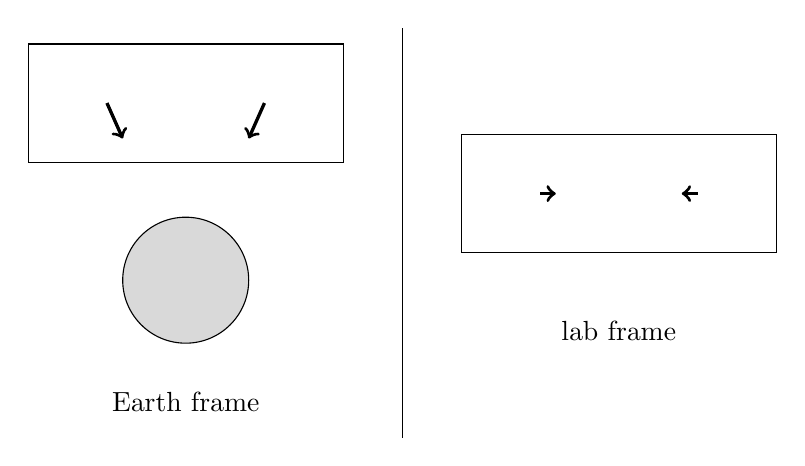
\begin{tikzpicture}
        \draw (0,0.5) rectangle (4,2);
        \draw[fill=gray!30] (2,-1) circle (0.8);
        \draw[->,very thick] (1,1.25) -- (1.2,0.8);
        \draw[->,very thick] (3,1.25) -- (2.8,0.8);
        \node[below] at (2,-2.3) {Earth frame};

        \draw (4.75,2.2) -- (4.75,-3);
    
        \draw (5.5,-0.65) rectangle (9.5,0.85);
        \draw[->,very thick] (6.5,0.1) -- (6.7,0.1);
        \draw[->,very thick] (8.5,0.1) -- (8.3,0.1);
        \node[below] at (7.5,-1.4) {lab frame};
    \end{tikzpicture}
\end{figure}
In the frame of the lab, \(\vb{g}\) varies significantly over the lab, so the lab frame is too ``large'' to be considered a local inertial frame.

The WEP was found in Newtonian physics. Einstein promoted it to be more general. The \emph{Einstein equivalence principle} is in two parts:
\begin{enumerate}
    \item The WEP is valid.
    \item In a local inertial frame, the results of all non-gravitational experiments are indistinguisable from those of the same experiment in an inertial frame in Minkowski spacetime.
\end{enumerate}

(``Schiff's conjecture'' is that the WEP implies the EEP, but this has not actually been proven.)

Henceforth we will assume the EEP.

\subsection{Bending of light}

Consider a freely falling laboratory in a uniform gravitational field. Inside the lab, light moves in a straight line, since the lab frame is a locally inertial one. Transforming to the Earth frame, we see that the light must take a curved path. It travels a horizontal distance given by \(d=ct\), and a vertical distance given by \(gt^2/2\). Hence the height of the light is given by \(h=\frac{gd^2}{2c^2}\) -- the light follows a parabola.

\subsection{Gravitational redshift}
Consider a uniform gravitational field \(\vb{g}=(0,0,-g)\) with two observers, Alice at \(z=h\) and Bob at \(z=0\). Alice sends light signals to Bob. The EEP implies that this is equivalent to a frame with acceleration \((0,0,g)\). We assume that \(v_A,v_B\ll c\), so that we can ignore \(\frac{v^2}{c^2}\) and higher order terms that arise from special relativity. In the accelerating frame we have
\begin{equation}
    z_A(t) = h + \frac12gt^2,\quad z_B(t) = \frac12gt^2,
\end{equation}
and \(v_A = v_B = gt \ll c\). Suppose Alice emits the first signal at \(t=t_1\). The path of the signal is given by
\begin{equation}
    z_1(t) = z_A(t_1) - c(t-t_1) = h+\frac12gt_1^2 - c(t-t_1).
\end{equation}
The signal reaches Bob at \(t=T_1\), defined by
\begin{equation}
    h+\frac12gt_1^2 - c(T_1-t_1) = \frac12gT_1^2.
\end{equation}
Now suppose Alice emits a second signal at \(t_2 = t_1 + \Delta\tau_A\) recieved by Bob at \(T_2 = T_1 + \Delta\tau_B\). Then we similarly have
\begin{equation}
    h+\frac12g(t_1+\Delta\tau_A)^2 - c(T_1 + \Delta\tau_B-t_1-\Delta\tau_A) = \frac12g(T_1+\Delta\tau_B)^2.
\end{equation}
Subtracting these equations we obtain
\begin{equation}
    c(\Delta\tau_A - \Delta\tau_B) + \frac12g\Delta\tau_A(2t_1 + \Delta\tau_A) = \frac12g\Delta\tau_B(2T_1+\Delta\tau_B).
\end{equation}
Now we assume that \(\Delta\tau_A\ll t_1\) and \(\Delta\tau_B\ll T_1\), as is the case for example when the signals are the consecutive peaks of light waves. Then we have
\begin{equation}
    c(\Delta\tau_A-\Delta\tau_B) + g\Delta\tau_At_1 = g\Delta\tau_BT_1,
\end{equation}
from which we can deduce
\begin{equation}
    \Delta\tau_B = \left(1+\frac{gT_1}{c}\right)^{-1}\left(1+\frac{gt_1}{c}\right)\Delta\tau_A \approx \left(1 - \frac{g(T_1-t_1)}{c}\right)\Delta\tau_A.
\end{equation}
Note that we have
\begin{equation}
    \frac{h}{c} - (T_1-t_1) = \frac12\underbrace{\frac{g}{c}(T_1+t_1)}_{\ll 1}\underbrace{(T_1-t_1)}_{\approx\frac{h}{c}} \approx 0,
\end{equation}
so to leading order \(T_1 - t_1 = \frac{h}{c}\). Therefore we have
\begin{equation}
    \Delta\tau_B \approx \left(1-\frac{gh}{c^2}\right)\Delta\tau_A.
\end{equation}
The signal appears blueshifted to Bob:
\begin{equation}
    c\Delta\tau_B = \lambda_B \approx \left(1-\frac{gh}{c^2}\right)\lambda_A
\end{equation}
This was confirmed in the Pound-Rebka experiment (1960). Similarly, light climbing out of a gravity well is redshifted. In general, we have
\begin{equation}
    \Delta\tau_B \approx \left(1+\frac{\phi_B-\phi_A}{c^2}\right)\Delta\tau_A.
\end{equation}
This equation holds for weak non-uniform fields.

\subsection{Curved spacetimes}
The WEP says that test bodies move in the same way in a gravitational field, regardless of their composition i.e.\ their gravitational ``charge'' \(m\). This is unlike any other force. Because of this, Einstein made the deduction that gravity must be a feature of spacetime, in particular its geometry.

Consider redshift but now in a non-Minkoskian metric
\begin{equation}
    c^2\dd{\tau}^2 = \left[1+\frac{2\phi(x,y,z)}{c^2}\right]c^2\dd{t}^2 - \left[1-\frac{2\phi(x,y,z)}{c^2}\right](\dd{x}^2+\dd{y}^2+\dd{z}^2),
\end{equation}
where \(\frac{\phi}{c^2}\ll1\). Alice and Bob are at fixed positions \(\vb{x}_A\) and \(\vb{x}_B\), and Alice emits signals at \(t_A\) and \(t_A+\Delta t\). Bob recieves the first signal at \(t_B\). When does he see the second one? Note that the spacetime is static (\(\phi\) is independent of \(t\)), so the 2 signals travel on identical trajectories, just shifted in time. Therefore Bob receives the second signal at \(t_B+\Delta t\) But what proper times do Alice and Bob measure? We have
\begin{equation}
    \Delta \tau_A^2 = \left(1+\frac{2\phi_A}{c^2}\right)\Delta t^2 \qq{and} \Delta\tau_B^2 = \left(1+\frac{2\phi_A}{c^2}\right)\Delta t^2,
\end{equation}
so we can write
\begin{equation}
    \Delta \tau_A \approx \left(1+\frac{\phi_A}{c^2}\right)\Delta t \qq{and} \Delta\tau_B \approx \left(1+\frac{2\phi_A}{c^2}\right)\Delta t,
\end{equation}
and we recover the above result:
\begin{equation}
    \Delta\tau_B \approx \left(1+\frac{\phi_B}{c^2}\right)\left(1+\frac{\phi_B}{c^2}\right)^{-1} \Delta\tau_A \approx \left(1+\frac{\phi_B-\phi_A}{c^2}\right)\Delta\tau_A
\end{equation}

\section{Manifolds and Tensors}

In GR we define spacetime as a manifold. This is trickier that just Minkowski spacetime for several reasons. In Minkowski spacetime, the presence of inertial frames leads to a preferred set of global coordinates, so we can add position vectors, and spacetime has the structure of a vector space. In a curved spacetime, inertial coordinates are local, and so we have no set of preferred coordinates, and it is not at first obvious how to interpret vectors.

\subsection{Differentiable manifolds}
We know how to do calculus in \(\RR^n\). The goal now is to develop an analog for curved spaces.

\begin{defn}
    An \(n\)-dimensional \emph{differentiable manifold} is a set \(\mathcal{M}\) with subsets \(\mathcal{O}_\alpha\) such that:
    \begin{enumerate}
        \item \(\bigcup_\alpha\mathcal{O}_\alpha=\mathcal{M}\).
        \item For all \(\alpha\) there is a bijection \(\phi_\alpha:\mathcal{O}_\alpha\to U_\alpha \subset\RR^n\), where \(U_\alpha\) is open.
        \item If \(\mathcal{O}_\alpha\cap\mathcal{O}_\beta \ne \varnothing\), then \(\phi_B\circ\phi_\alpha^{-1}:\phi_\alpha(\mathcal{O}_\alpha\cap\mathcal{O}_\beta) \to \phi_\beta(\mathcal{O}_\alpha\cap\mathcal{O}_\beta)\) is a smooth map. 
    \end{enumerate}
\end{defn}

The \(\phi_\alpha\) are sometimes called \emph{charts}, and the set of all charts for a manifold is sometimes called its \emph{atlas}. For \(p\in\mathcal{O}_\alpha\), we often write
\begin{equation}
    \phi_\alpha(p) = (x^1_\alpha(p),x_\alpha^2(p),x_\alpha^3(p),\dots) = x_\alpha^\mu(p).
\end{equation}
These are the \emph{coordinates} of \(p\); the \(\alpha\) is often dropped. 

A \(C^k\) manifold is defined likewise. From now on we'll assume that all our manifolds are \(C^\infty\).

\begin{eg}
    \begin{itemize}
        \item \(\RR^n\) is a manifold with an atlas of one chart \(\phi:(x_1,\dots,x_n)\mapsto(x_1,\dots,x_n)\).
        \item \(S^1 = \{(\cos\theta,\sin\theta)\in\RR^2 \st \theta \in \RR\}\), the unit circle, is a manifold. There does not exist an atlas for \(S^1\) with only one chart. We need two charts. Let \(P=(1,0)\) and \(Q=(-1,0)\). Then two possible such charts are \(\phi_1:S^1\setminus\{P\}\to(0,2\pi),p \mapsto \theta\) and \(\phi_2:S^1\setminus\{Q\}\to(-\pi,\pi),p\mapsto \theta\).
    \end{itemize}
\end{eg}

\begin{defn}
    Two atlases are \emph{compatible} iff their union is also an atlas. A \emph{complete} atlas is the union of all atlases compatible with a given atlas.
\end{defn}

\subsection{Smooth functions}
\begin{defn}
    A function \(f:\mathcal{M}\to\RR\) is smooth provided that for all charts \(\phi\) the function \(F=f\circ\phi^{-1}:U\subset\RR^n\to\RR\) is smooth.
\end{defn}
Sometimes we call \(f\) a \emph{scalar field}.
\begin{eg}
    \begin{itemize}
        \item For \(S^1\) above, \(f:S^1\to\RR,(x,y)\mapsto x\) is a smooth function.
        \item Consider a manifold \(\mathcal{M}\) with a chart \(\phi:\mathcal{O}\subset\mathcal{M}\to U\subset\RR^n, p\in\mathcal{O}\mapsto (x^1(p),\dots,x^n(p))\). Let \(f:\mathcal{O}\to\RR,p\mapsto x_1(p)\). Then \(f\) is smooth.
        \item We can define \(f\) through \(F\). Given an atlas \(\{\phi_\alpha\}\) then a set of \(F_\alpha:U_\alpha \to \RR\) defines \(f = F_\alpha\circ\phi_\alpha\), provided \(F_\alpha\) is independent of \(\alpha\) on overlapping regions. Note that since we can go easily between \(f\) and \(F\) we sometimes abuse notation and do not distinguish them.
    \end{itemize}
\end{eg}

\subsection{Curves and vectors}
Consider a surface in \(\RR^3\), and the tangent plane at a point \(p\) in that surface. The plane has the structure of a 2D vector space, and a tangent vector to a curve in the surface at \(p\) is in the plane. The goal in this section is to formalise this for an \(n\)-manifold.

\begin{defn}
    A smooth curve in a manifold \(\mathcal{M}\) is a function \(\lambda:I\to\mathcal{M}\) where \(I\subset\RR\) is open, such that \(\phi_\alpha\circ\lambda:I\to\RR^n\) is smooth for all charts \(\phi_\alpha\).
\end{defn}
\begin{defn}
    Let \(\mathcal{C}^\infty(\mathcal{M},\RR)\) be the space of all smooth functions from \(\mathcal{M} \to \RR\), and let \(\lambda\) be a smooth curve with \(\lambda(0) = p \in \mathcal{M}\). The \emph{tangent vector} to \(\lambda\) at \(p\) is the linear map
    \begin{equation}
        \fullfunction{X_p}{\mathcal{C}^\infty(\mathcal{M},\RR)}{\RR}{f}{X_p(f) = \left.\dv{t}f(\lambda(t))\right|_{t=0}}.
    \end{equation}
\end{defn}
Tangent vectors are linear and obey the Leibniz rule:
\begin{equation}
    X_p(f+g) = X_p(f) + X_p(g),\quad X_p(\alpha f) = \alpha X_p(f),\quad X_p(fg) = X_p(f)g(0) + X_p(g)f(0)
\end{equation}
Suppose \(\phi=(x^\mu)\) is a chart defined in a neighbourhood of \(p \in \mathcal{M}\) and let \(F=f\circ\phi^{-1}\). Then we have
\begin{align}
    f\circ \lambda &= (f\circ\phi^{-1}) \circ (\phi\circ\lambda) = F\circ\phi\circ\lambda, \\
    X_p(f) &= \left.\dv{t}(F\circ\phi\circ\lambda)(t)\right|{t=0} \\
           &= \left(\dv{F}{x^\mu}\right)_{\phi(p)} \left(\dv{x^\mu(\lambda(t))}{t}\right)_{t=0} \\
           &= \dv{x^\mu}{t}\pdv{x^\mu} F \\
           &= \dv{t} F(x^\mu(\lambda(t))) = \dv{t}(f(\lambda(t))).
\end{align}
For this reason, we call \(\dv{x^\mu}{t}\) the components of the vector, expanded in the basis \(\pdv{x^\mu}\). We also just refer to \(\dv{t}\) itself as the vector.

\begin{lemma}
    The set of vectors at \(p\in\mathcal{M}\) form an \(n\)-dimensional vector space (known as the \emph{tangent space} \(\mathcal{T}_p(\mathcal{M})\)).
\end{lemma}
The proof is simple.

Note that \(\left(\pdv{x^\mu}\right)_p\) is not the same as the partial derivative \(\pdv{^\mu}\). Also, the basis \(\left(\pdv{x^\mu}\right)_p\) is chart dependent, so we call it the \emph{coordinate basis}.

\begin{defn}
    Let \(\{e_\mu\}\) be a basis of \(\mathcal{T}_p(\mathcal{M})\). Then we can expand any vector in this basis, \(X_p = X_p^\mu e_\mu\). \(X_p^\mu\) are the \emph{components} of \(X_p\).
\end{defn}
\begin{eg}
    For a coordinate basis, we have \(X_p^\mu = \left(\dv{x^\mu(\lambda(t))}{t}\right)_{t=0}\).
\end{eg}
Note that when Einstein convention is applied, we always have one index up and one down (and we take e.g.\ \(\pdv{x^\mu}\) to be a ``down index'').

Let \(\phi=(x^\mu)\) and \(\bar\phi = (\bar{x}^\mu)\) be two charts in a neighbourhood of \(p\in \mathcal{M}\). Then we have
\begin{align}
    \left(\pdv{x^\mu}\right)_p(f) &= \left.\pdv{x^\mu}(f\circ\phi^{-1})\right|_{\phi(p)} \\
                                  &= \pdv{x^\mu}\Big[(f\circ\bar\phi^{-1})\circ\underbrace{(\bar\phi\circ\phi^{-1})}_{=\bar{x}^\mu(x^\alpha)}\Big]\Bigg|_{\phi(p)} \\
                                  &= \left.\pdv{x^\mu}\left[(f\circ\bar\phi^{-1})(\bar{x}(x))\right]\right|_{p} \\
                                  &= \left[\pdv{\bar{x}^\alpha}(f\circ\bar\phi^{-1})\right]_{\bar\phi(p)}\left.\pdv{\bar{x}^\alpha}{x^\mu}\right|_{\phi(p)} \\
                                  &= \left(\pdv{\bar{x}^\alpha}\right)_p(f) \left.\pdv{\bar{x}^\alpha}{x^\mu}\right|_{\phi(p)} \\
    \implies \left(\pdv{x^\mu}\right)_p &= \left(\pdv{\bar{x}^\alpha}{x^\mu}\right)_{\phi(p)}\left(\pdv{\bar{x}^\alpha}\right)_p.
\end{align}

Using this, we can see how the components of a vector transforms when changing between charts. Consider a vector \(V \in \mathcal{T}_p(\mathcal{M})\). We have
\begin{equation}
    V = V^\mu\left(\pdv{x^\mu}\right)_p = V^\mu\left(\pdv{\bar{x}^\alpha}{x^\mu}\right)_{\phi(p)}\left(\pdv{\bar{x}^\alpha}\right)_p = \bar{V}^\alpha\left(\pdv{\bar{x}^\alpha}\right)_p,
\end{equation}
where \(\bar{V}^\alpha = \left(\pdv{\bar{x}^\alpha}{x^\mu}\right)_{\phi(p)}V^\mu\). Vector components transform \emph{contravariantly}.

\subsection{Covectors/1-forms}
\begin{defn}
    Let \(\mathcal{V}\) be an \(n\)-dimensional vector space over \(\RR\). Its \emph{dual space} \(\mathcal{V}^*\) is the \(n\)-dimensional vector space of linear maps \(\mathcal{V}\to\RR\). If \(\{e_\mu\}\) is a basis of \(\mathcal{V}\), then the \emph{dual basis}, a basis of \(\mathcal{V}^*\) is \(\{f^\alpha\}\), defined by \(f^\alpha(e_\mu) = \delta^\alpha_\mu\).
\end{defn}

\(\mathcal{V}\) and \(\mathcal{V}^*\) are isomorphic. For example \(e_\mu \mapsto f^\mu\) defines an isomorphism. However it is important to note that this isomorphism must be basis dependent. On the other hand:
\begin{theorem}
    If \(\mathcal{V}\) is finite dimensional, then a natural, basis independent isomorphism between \(\mathcal{V}\) and \((\mathcal{V}^*)^*\) is given by \(\Phi:\mathcal{V}\to(\mathcal{V}^*)^*,X\mapsto\Phi(X)\), where \((\Phi(X))(\omega)=\omega(X)\) for all \(\omega \in \mathcal{V}^*\).
\end{theorem}

\begin{defn}
    The \emph{cotangent space} \(\mathcal{T}^*_p(\mathcal{M})\) is the dual space of \(\mathcal{T}_p(\mathcal{M})\). Its elements are called \emph{covectors} or \emph{1-forms}. If \(\{e_\mu\}\) is a basis of \(\mathcal{T}_p(\mathcal{M})\) and \(\{f^\mu\}\) is its dual basis in \(\mathcal{T}_p^*(\mathcal{M})\), then the components \(\eta_\mu\) of a 1-form \(\eta\) in this basis are defined by \(\eta = \eta_\mu f^\mu\).
\end{defn}

Note that \(\eta(e_\mu) = \eta_\nu f^\nu(e_\mu) = \eta_\nu\delta^\nu_\mu = \eta_\mu\). Consequently, if \(X \in \mathcal{T}_p(\mathcal{M})\), then \(\eta(X) = \eta(X^\mu e_\mu) = X^\mu\eta(e_\mu) = X^\mu\eta_\mu\).

\begin{defn}
    Let \(f:\mathcal{M}\to\RR\) be a smooth function. Then the \emph{gradient} of \(f\) at \(p\) is the 1-form \((\dd{f})_p\) defined by \((\dd{f})_p(X) = X(f)\) for all \(X \in \mathcal{T}_p(\mathcal{M})\).
\end{defn}
Let \((x^i)\) be a coordinate chart in a neighbourhood of \(p\in\mathcal{M}\). Then \((\dd{x^\mu})_p\in\mathcal{T}^*_p(\mathcal{M})\) has the property that \((\dd{x^\mu})_p\left(\left(\pdv{x^\nu}\right)_p\right) = \left.\pdv{x^\mu}{x_\nu}\right|_p = \delta^\mu_\nu\). Hence \(\{(\dd{x^\mu})_p\}\) is the dual basis of \(\left\{\left(\pdv{x^\mu}\right)_p\right\}\).

The coefficients of \((\dd{f})_p\) are given by
\begin{equation}
    \left[(\dd{f})_p\right]_\mu = (\dd{f})_p\left(\left(\pdv{x^\mu}\right)_p\right) = \left(\pdv{x^\mu}\right)_p(f) = \left(\pdv{F}{x^\mu}\right)_{\phi(p)}.
\end{equation}
If \(\phi=(x^\mu)\) and \(\bar\phi=(\bar{x}^\mu)\) are two charts in a neighbourhood of \(p\in \mathcal{M}\), then we can carry out a similar series of steps as with vectors to obtain
\begin{equation}
    (\dd{x^\mu})_p = \left(\pdv{x^\mu}{\bar{x}^\nu}\right)_{\bar\phi(p)}(\dd{\bar{x}^\nu})_p.
\end{equation}
Hence for \(\omega \in \mathcal{T}_p^*(\mathcal{M})\), we can write \(\omega = \omega\dd{x^\mu} = \bar{\omega}_\mu\dd{\bar{x}^\mu}\), where \(\bar\omega_\mu = \left(\pdv{x^\nu}{\bar{x}^\mu}\right)_{\bar\phi(p)}\omega_\nu\). Covector components transform \emph{covariantly}.

\subsection{Abstract index notation}
We have been using Greek indices \(\mu,\nu,\dots\) for components of vectors and 1-forms in a basis. This is appropriate for when expressions are basis dependent, but sometimes they are not. For example, while \(X^\mu = \delta_1^\mu\) is basis dependent, \(\eta(X) = \eta_\mu X^\mu\) is not. 

If a statement is true in any basis we replace \(\mu,\nu,\dots\) with early Latin letters \(a,b,\dots\), and define expressions by their equivalent basis independent forms. For example \(\eta_aX^a \equiv \eta(X)\). Conventionally, \(a,b,\dots\) do \emph{not} denote components, but rather placeholders for components indices. 

\(X^a\) is a vector, \(\eta_a\) is a 1-form, but \(X^\mu\) are the components of a vector, and so on.

The rules for index positions are the same as for \(\mu,\nu,\dots\).

\subsection{Tensors}
\begin{defn}
    A \emph{tensor} of type \((r,s)\) is a multilinear map
    \begin{equation}
        T:\underbrace{\mathcal{T}^*_p(\mathcal{M})\times\dots\times\mathcal{T}^*_p(\mathcal{M})}_{r} \times \underbrace{\mathcal{T}_p(\mathcal{M})\times\dots\times\mathcal{T}_p(\mathcal{M})}_s \to \RR.
    \end{equation}
\end{defn}
\begin{eg}
    \begin{itemize}
        \item A 1-form is a \((0,1)\) tensor.
        \item Recall that \((\mathcal{T}_p^*(\mathcal{M}))^*\) is naturally isomorphic to \(\mathcal{T}_p(\mathcal{M})\), so a vector is a \((1,0)\) tensor.
            \begin{equation}
                V:\mathcal{T}_p^*(\mathcal{M})\to\RR,\quad \eta \to \eta(V) \forall \eta \in \mathcal{T}^*_p(\mathcal{M})
            \end{equation}
        \item We define the \((1,1)\) tensor \(\delta:\mathcal{T}^*_p(\mathcal{M})\times\mathcal{T}_p(\mathcal{M})\to\RR\) through \(\delta(\eta,X) = \eta(X)\) for all \(\eta \in \mathcal{T}_p^*(\mathcal{M})\) and \(X \in \mathcal{T}_p(\mathcal{M})\).
    \end{itemize}
\end{eg}

\begin{defn}
    Let \(\{e_\mu\}\) be a basis of \(\mathcal{T}_p(\mathcal{M}\), and let \(\{f^\mu\}\) be its dual basis in \(\mathcal{T}^*_p(\mathcal{M})\). Then the \emph{components} of an \((r,s)\) tensor \(T\) are given by
    \begin{equation}
        T\indices{^{\mu_1\dots\mu_r}_{\nu_1\dots\nu_s}} = T(f^{\mu_1},\dots,f^{\mu_r},e_{\nu_1},\dots,e_{\nu_s}).
    \end{equation}
\end{defn}

Tensors of type \((r,s)\) at \(p\in\mathcal{M}\) can be added or multiplied with constants. One can show that they form a vector space of dimension \(n^{r+s}\).
\begin{eg}
    \begin{itemize}
        \item The components of \(\delta\) are \(\delta(f^\mu,e_\nu) = f^\mu(e_\nu) = \delta^\mu_\nu\).
        \item Let \(\eta,\omega\in\mathcal{T}_p^*(\mathcal{M}\), \(X\in \mathcal{T}_p(\mathcal{M})\) and \(T\) a \((2,1)\) tensor. Then
            \begin{align}
                T(\eta,\omega,X) &= T(\eta_\mu f^\mu,\omega_\nu f^\nu,X^\alpha e_\alpha) \\
                                 &= \eta_\mu\omega_\nu X^\alpha T(f^\mu,f^\nu,e_\alpha) \\
                                 &= \eta_\mu\omega_\nu X^\alpha T\indices{^{\mu\nu}_\alpha},
            \end{align}
            or in abstract index notation, \(\eta_a\omega_b X^c T\indices{^{ab}_c}\).
    \end{itemize}
\end{eg}

Let \(\{e_\mu\}\) and \(\{\bar{e}_\nu\) be bases of \(\mathcal{T}_p(\mathcal{M})\), and let \(\{f^\mu\}\) and \(\{\bar{f}^\nu\}\) be the corresponding dual bases of \(\mathcal{T}_p^*(\mathcal{M})\). We can expand the barred basis in terms of the unbarred one, writing
\begin{equation}
    \bar{f}^\mu = A\indices{^\mu_\nu} f^\nu \qq{and} \bar{e}_\mu = B\indices{^\nu_\mu}e_\nu.
\end{equation}
Then we have
\begin{align}
    \delta^\mu_\nu &= \bar{f}^\mu(\bar{e}_\nu) \\
                   &= A\indices{^\mu_\rho} f^\rho(B\indices{^\sigma_\nu}e_\sigma) \\
                   &= A\indices{^\mu_\rho}B\indices{^\sigma_\nu} \underbrace{f^\rho(e_\sigma)}_{=\delta^\rho_\sigma} \\
                   &= A\indices{^\mu_\rho}B\indices{^\rho_\nu}.
\end{align}
Hence \(B\indices{^\mu_\nu} = (A^{-1})\indices{^\mu_\nu}\), i.e.\ \(B\) and \(A\) are inverses of each other. For example, in a coordinate basis,
\begin{equation}
    A\indices{^\mu_\nu} = \pdv{\bar{x}^\mu}{x^\nu} \qq{and} B\indices{^\nu_\mu} = \pdv{x^\nu}{\bar{x}^\mu}
\end{equation}
are obviously inverses.

We have shown that if vector components transform as \(\bar{X}^\mu = A\indices{^\mu_\nu}X^\nu\), then covector components transform as \(\bar{\eta}_\mu = (A^{-1})\indices{^\nu_\mu}\eta_\nu\). This naturally extends to \((r,s)\) tensors, where we have \(r\) \(A\)s and \(s\) \(A^{-1}\)s; for example for a \((2,1)\) tensor we have
\begin{equation}
    \bar{T}\indices{^{\mu\nu}_\rho} = A\indices{^\mu_\alpha}A\indices{^\nu_\beta}(A^{-1})\indices{^\gamma_\rho}T\indices{^{\alpha\beta}_\gamma}.
\end{equation}

\begin{defn}
    \emph{Contraction} of an \((r,s)\) tensor is summation over one upper and one lower index, and gives a \((r-1,s-1)\) tensor.
\end{defn}

\begin{eg}
    Let \(T\) be a \((3,2)\) tensor, and let \(S\) be a \((2,1)\) tensor defined by
    \begin{equation}
        S(\omega,\eta,X) = \sum_\nu T(f^\nu,\omega,\eta,e_\nu,X).
    \end{equation}
    This is basis independent:
    \begin{align}
        T(\bar{f}^\mu,\omega,\eta,\bar{e}_\mu,X) &= T(A\indices{^\mu_\nu}f^\nu,\omega,\eta,(A^{-1})\indices{^\rho_\mu}e_\rho,X) \\
                                                 &= T(f^\nu,\omega,\eta,e_\mu,X)
    \end{align}
    The components of \(S\) are \(S\indices{^{\mu\nu}_\rho} = \sum_\alpha T\indices{^{\alpha\mu\nu}_{\alpha\rho}}\). Because we have basis independence, we can use abstract index notation: \(S\indices{^{ab}_c} = T\indices{^{dab}_{dc}}\).
\end{eg}

\begin{defn}
    Let \(S\) be a \((p,q)\) tensor, and \(T\) a \((r,s)\) tensor. The \emph{outer product} of \(S\) and \(T\) is a \((p+r,q+s)\) tensor \(S\otimes T\) defined by
    \begin{multline}
        (S\otimes T)(\omega_1,\dots,\omega_p,\eta_1,\dots,\eta_r,X_1,\dots,X_q,Y_1,\dots,Y_s) \\
        = S(\omega_1,\dots,\omega_p,X_1,\dots,X_q)T(\eta_1,\dots,\eta_r,Y_1,\dots,Y_s).
    \end{multline}
\end{defn}
One can show
\begin{equation}
    (S\otimes T)\indices{^{a_1\dots a_p b_1\dots b_r}_{c_1\dots c_q d_1\dots d_s}} = S\indices{^{a_1\dots a_p}_{c_1\dots c_q}} T\indices{^{b_1\dots b_r}_{d_1\dots d_s}}.
\end{equation}

\begin{eg}
    In a coordinate basis, a \((2,1)\) tensor can be written
    \begin{equation}
        T = T\indices{^{\mu\nu}_\rho}\left(\pdv{x^\mu}\right)_p\otimes\left(\pdv{x^\nu}\right)_p\otimes(\dd{x^\rho})_p.
    \end{equation}
    Likewise with an \((r,s)\) tensor.
\end{eg}

\begin{defn}
    Let \(T\) be a \((0,2)\) tensor. The \emph{symmetrisation} \(S\) of \(T\) is defined by
    \begin{equation}
        S_{ab} = \frac12(T_{ab}+T_{ba}).
    \end{equation}
    We write \(S_{ab} = T_{(ab)}\). The \emph{anti-symmetrisation} \(A\) of \(T\) is defined by
    \begin{equation}
        A_{ab} = \frac12(T_{ab}-T_{ba}).
    \end{equation}
    We write \(A_{ab} = T_{[ab]}\). We can apply this to a subset of indices of a higher rank tensor, for example
    \begin{equation}
        T\indices{^{(ab)c}_d} = \frac12(T\indices{^{abc}_d} + T\indices{^{bac}_d}).
    \end{equation}
    We can also do this over more than two indices, in which case we sum over all permutations (applying the sign of the permutation to each term if anti-symmetrising), and divide by \(n!\). For example
    \begin{equation}
        T\indices{^a_{[bcd]}} = \frac16(T\indices{^a_{bcd}} + T\indices{^a_{cdb}} + T\indices{^a_{dbc}} 
        - T\indices{^a_{bdc}} - T\indices{^a_{dcb}} - T\indices{^a_{cbd}}).
    \end{equation}
    There is also a notation for skipping non-adjacent indices:
    \begin{equation}
        T_{(a|bc|d)} = \frac12(T_{abcd}+T_{dbca})
    \end{equation}
\end{defn}

\subsection{Tensor fields}
So far, we have only defined tensors at fixed points \(p\in \mathcal{M}\). Now we generalise to fields.
\begin{defn}
    A \emph{vector field} is a map \(X:\mathcal{M}\to\mathcal{T}_p(\mathcal{M}),p\mapsto X_p\) (Technically this is nonsense; a vector field is actually a section of the tangent bundle). Let \(f:\mathcal{M}\to\RR\) be a smooth function. Then \(X(f):\mathcal{M}\to\RR,p\mapsto X_p(f)\) is a function. We say that \(X\) is \emph{smooth} iff \(X(f)\) is smooth for all smooth \(f\).
\end{defn}

\begin{eg}
    Let \(x^\mu\) be a chart and write \(\partial_\mu = \left(\pdv{x^\mu}\right)\). Then \(\partial_\mu f : \mathcal{M}\to\RR, p\mapsto \left(\pdv{F}{x^\mu}\right)_{x^\mu(p)}\), where \(F = f\circ\phi^{-1}\), \(\phi = (x^\mu)\), is a vector field. If \(\phi\), \(F\) and \(\pdv{F}{x^\mu}\) are smooth, then \(\partial_\mu f\) is smooth.
\end{eg}
Recall that \(\left(\pdv{x^\mu}\right)_p\) is a basis of \(\mathcal{T}_p(\mathcal{M}\). We can therefore expand the vector field \(X=X^\mu\pdv{x^\mu}=X^\mu\partial_\mu\). Since \(\partial_\mu\) is smooth, we have that \(X\) is smooth iff \(X^\mu\) are smooth functions.
\begin{defn}
    A \emph{covector field} is a map \(\omega:\mathcal{M}\to\mathcal{T}_p^*(\mathcal{M}),p\mapsto\omega_p\). A vector field \(X\) and covector field \(\omega\) together define a function \(\omega(X):\mathcal{M}\to\RR, p\mapsto\omega_p(X_p)\). \(\omega\) is \emph{smooth} iff \(\omega(X)\) is smooth for all smooth \(X\).
\end{defn}

\begin{eg}
    Let \(f\) be a function. Then the gradient field is \(\dd{f}:\mathcal{M}\to\mathcal{T}_p^*(\mathcal{M}),p\mapsto(\dd{f})_p\). If \(f\) and \(X\) are smooth, then \(\dd{f}(X)=X(f)\) is also smooth, so \(\dd{f}\) is smooth. If we set \(f=x^\mu\), then we get a smooth coordinate basis for covector fields \(\dd{x^\mu}\) (in general only locally).
\end{eg}

\begin{defn}
    An \((r,s)\) \emph{tensor field} is a map \(T:\mathcal{M}\to\text{\((r,s)\) tensor at \(p\in\mathcal{M}\)}\). Its smoothness is defined similarly to above.
\end{defn}
Note that \(T\) is smooth iff its components are smooth. From now on, we will assume that all tensors we deal with our smooth.

\subsection{The commutator}
Let \(X,Y\) be two vector fields, and \(f,g\) be functions. Then \(Y(f)\) is a function, and hence so is \(X(Y(f))\). However,
\begin{align}
    X(Y(fg)) &= X(fY(g) + gY(f)) \\
             &= fX(Y(g)) + gX(Y(f)) + X(f)Y(g)+X(g)Y(f) \\
             &\ne fX(Y(g)) + gX(Y(f)),
\end{align}
which is what we would expect if \(XY\) satisfied the Leibniz rule. Hence the map \(f\mapsto X(Y(f))\) does not define a vector field. But:
\begin{defn}
    The \emph{commutator} \([X,Y]\) of two vector fields \(X\) and \(Y\) is defined by
    \begin{equation}
        [X,Y](f) = X(Y(f)) - Y(X(f)).
    \end{equation}
\end{defn}
The commutator satisfies the Leibniz rule as the extra terms above cancel. Furthermore, \([X,Y]\) is a bonafide vector field, and we can prove this by looking at its components in a coordinate chart \((x^\mu)\). We have
\begin{align}
    [X,Y](f) &= X^\mu\pdv{x^\mu}\left(Y^\nu\pdv{F}{x^\nu}\right) - Y^\nu\pdv{x^\nu}\left(X^\mu\pdv{F}{x^\mu}\right) \\
             &= X^\mu\pdv{Y_\nu}{x^\mu}\pdv{F}{x^\nu} - Y^\nu\pdv{X^\mu}{x^\nu}\pdv{F}{x^\mu}
                + X^\mu Y^\nu\pdv[2]{F}{x^\mu}{x^\nu} - X^\mu Y^\nu\pdv[2]{F}{x^\mu}{x^\nu} \\
             &= \underbrace{\left(X^\nu\pdv{Y^\mu}{x^\nu}-Y^\nu\pdv{X^\mu}{x^\nu}\right)}_{=[X,Y]^\mu}\pdv{F}{x^\mu}.
\end{align}
Since \(f\) was arbitrary, we can thus write \([X,Y] = [X,Y]^\mu\pdv{x^\mu}\), which is obviously a vector.

\begin{eg}
    Let \(X=\pdv{x^1}\) and \(Y = x^1\pdv{x^2} + \pdv{x^3}\). Then \([X,Y]^\mu = \pdv{Y^\mu}{x^1} = \delta^\mu_2\), so \([X,Y] = \pdv{x^2}\).
\end{eg}
One can show the following:
\begin{equation}
    [X,Y]=-[Y,X],\quad
    [X,Y+Z] = [X,Y] + [X,Z],\quad
    [X,fY] = f[X,Y] + X(f)Y
\end{equation}
The commutator also satisfies the Jacobi identity:
\begin{equation}
    [X,[Y,Z]] + [Y,[Z,X]] + [Z,[X,Y]] = 0
\end{equation}
Note that \(\left[\pdv{x^\mu},\pdv{x^\nu}\right] = 0\). Conversely, one can show that if \(X_1,\dots,X_m\), \(m\le\dim\mathcal{M}\) are vector fields which are linearly independent at all points \(p\in\mathcal{M}\) and whose commutators \emph{all} vanish, then in a neighbourhood of \(p\) one can find coordinates \((x^\mu)\) such that \(X_i = \pdv{x^i}\), \(i=1,\dots,m\).

\subsection{Integral curves}
\begin{defn}
    Let \(X\) be a vector field, and \(p\in\mathcal{M}\). The \emph{integral curve} of \(X\) through \(p\) is defined as the curve through \(p\) whose tangent vector at every point \(q\) (on the curve) is \(X_q\).
\end{defn}

Let \(\lambda\) be an integral curve of \(X\) with \(\lambda(0) = p\), and \((x^\mu)\) be a coordinate chart. Then we have
\begin{equation}
    \dv{x^\mu(\lambda(t))}{t} = X^\mu(x^\alpha(\lambda(t))) \qq{and} x^\mu(\lambda(0)) = x^\mu_p.
\end{equation}
ODE theory guarantees the existence and uniqueness of a solution. Therefore the integral curve of \(X\) through \(p\in \mathcal{M}\) exists and is unique.
\begin{eg}
    Let \(X = \pdv{x^1} + x^1\pdv{x^2}\), and \(x^\mu(p) = (0,\dots,0)\). Then we have
    \begin{equation}
        \dv{x^1}{t} = 1,\quad \dv{x^2}{t} = x^1,
    \end{equation}
    which has solution
    \begin{equation}
        x^1=t,\quad x^2=\frac12 t^2,\quad x^i=0 \;\text{for}\; i > 2.
    \end{equation}
\end{eg}

\section{The Metric Tensor}
We want to be able to measure things, and to do so we need a metric. To see what form this metric should take, notice that in \(\RR^n\) we have a scalar product to do the job, mapping two vectors to a number in \(\RR\). By analogy, the metric should be a \((0,2)\) tensor.

\begin{defn}
    A metric at \(p\in \mathcal{M}\) is a \((0,2)\) tensor that is:
    \begin{itemize}
        \item Symmetric: \(g(X,Y) = g(Y,X)\) for all \(X,Y\in\mathcal{T}_p(\mathcal{M})\), i.e.\ \(g_{ab} = g_{ba}\).
        \item Non-degenerate: \(g(X,Y) = 0 \,\Forall\, Y\in\mathcal{T}_p(\mathcal{M}) \iff X=0\).
    \end{itemize}
\end{defn}

There are several alternate notations for the metric:
\begin{equation}
    g(X,Y) = \expval{X,Y} = X\vdot Y
\end{equation}

A metric defines an isomorphism between vectors and 1-forms, given by \(X\mapsto g(X,\cdot)\). Hence we can use the metric to raise and lower indices.

Since \(g\) is symmetric, the components of \(g\) at \(p\in\mathcal{M}\) are a symmetric matrix, so there is a basis in which \(g_{\mu\nu}\) is diagonal. Furthermore, since \(g\) is non-degenerate, all of the diagonal elements in this basis are non-zero. Hence we can rescale the basis such that the diagonal elements are \(\pm1\); such a basis is called \emph{orthonormal}. \emph{Sylvester's law} is the statement that the number of positive and negative diagonal elements is basis independent, so we can define:
\begin{defn}
    The \emph{signature} of a metric is the sum over all diagonal elements in the orthonormal basis.
\end{defn}
\begin{defn}
    A \emph{Riemannian metric} is one with signs \(+\dots+\), or signature \(n=\dim\mathcal{M}\). A \emph{Lorentzian metric} is one with signs \(-+\dots+\), or signature \(n-2\).
\end{defn}

Note that the equivalence principle gives us that in a local intertial frame the laws of special relativity hold, so there must exist a chart where locally \(g_{\mu\nu}=\eta_{\mu\nu} = \operatorname{diag}(-1,+1,+1,+1)\). This is only possible locally; at \(q\ne p\), \(g_{\mu\nu}\ne\eta_{\mu\nu}\) in general.

\begin{defn}
    A \emph{Riemannian (Lorentzian) manifold} is a tuple \((\mathcal{M},g)\) where \(\mathcal{M}\) is a differentiable manifold and \(g\) is a Riemannian (Lorentzian) metric on \(\mathcal{M}\).
\end{defn}

In a coordinate basis we have \(g=g_{\mu\nu}\dd{x^\mu}\otimes\dd{x^\nu}\). We will often notate this in terms of the ``line element'' \(\dd{s}^2=g_{\mu\nu}\dd{x^\mu}\dd{x^\nu}\).

Let \(\lambda:(a,b)\subset\RR\to\mathcal{M}\) be a smooth curve on a Riemannian manifold with tangent \(X\). The ``length'' of \(\lambda\) is given by
\begin{equation}
    s = \int_a^b\sqrt{g(X,X)_{\lambda(t)}} \dd{t}.
\end{equation}
The length is invariant under reparametrisation of the curve.

\begin{eg}
    \begin{itemize}
        \item The Euclidean metric in \(\RR^n\) with coordinates \(x^1,\dots,x^n\) is defined by
            \begin{equation}
                g = \dd{x^1}\otimes\dd{x^1} + \dots + \dd{x^n}\otimes\dd{x^n}.
            \end{equation}
            A coordinate chart of \((\RR^n,g)\) where \(g_{\mu\nu} = \operatorname{diag}(1,\dots,1)\) is called Cartesian.
        \item The Minkowski metric in \(\RR^n\) with coordinates \(x^0,x^1,x^2,x^3\) is defined by
            \begin{equation}
                \eta = -(\dd{x^0})^2 + (\dd{x^1})^2 + (\dd{x^2})^2 + (\dd{x^3})^2,
            \end{equation}
            where \((\dd{x^\mu})^2 = \dd{x^\mu}\otimes\dd{x^\mu}\). A coordinate chart which covers \(\RR^4\) such that \(\eta_{\mu\nu} = \operatorname{diag}(-1,1,1,1)\) is called an inertial frame, and \((\RR^4,\eta)\) is Minkowski spacetime.
        \item Let \((\theta,\phi)\) be spherical coordinates on \(S^2\) and consider the spherical metric given by
            \begin{equation}
                \dd{s}^2 = \dd{\theta}^2 + \sin^2\theta\dd{\phi}^2.
            \end{equation}
            This is only non-degenerate on \(\theta\in (0,\pi)\), reflecting the fact that we need a second coordinate chart to complete the sphere.
    \end{itemize}
\end{eg}

Since \(g\) is non-degenerate, it is invertible.
\begin{defn}
    The \emph{inverse metric} \(g^{-1}\) is a symmetric \((2,0)\) tensor \(g^{ab}\) with \(g^{ab}g_{bc} = \delta^a_c\).
\end{defn}
\begin{eg}
    For the third example above, \(g^{\mu\nu} = \operatorname{diag}\left(1,\frac1{\sin^2\theta}\right)\).
\end{eg}
\(g^{-1}\) maps 1-forms to vectors. The metric mappings between vectors and 1-forms are inverses of each other, so now we have a natural isomorphism between the two.

\subsection{Lorentzian signature}
At any \(p\in\mathcal{M}\) of a Lorentzian manifold, we can choose an orthonormal basis \(e_\mu\) in which \(g(e_\mu,e_\nu) = \eta_{\mu\nu} = \operatorname{diag}(-1,1,\dots,1)\). This basis is not unique; suppose we chose another basis \(\bar{e}_\mu = (A^{-1})\indices{^\nu_\mu}e_\nu\). Then the components of the metric in this basis are
\begin{equation}
    \bar{g}_{\mu\nu} = g(\bar{e}_\mu,\bar{e}_\nu) = (A^{-1})\indices{^\rho_\mu}(A^{-1})\indices{^\sigma_\nu}g(e_\rho,e_\sigma) = (A^{-1})\indices{^\rho_\mu}(A^{-1})\indices{^\sigma_\nu} \eta_{\rho\sigma}.
\end{equation}
If the new basis is also orthonormal so that \(\bar{g}_{\mu\nu} = \eta_{\mu\nu}\), then we have
\begin{equation}
    A\indices{^\mu_\rho}A\indices{^\nu_\sigma} = \eta_{\rho\sigma},
\end{equation}
so \(A\) is just a Lorentz transform. Hence orthornormal bases are related by Lorentz transforms and locally at \(p\in \mathcal{M}\) we recover special relativity.
\begin{defn}
    Let \((\mathcal{M},g)\) be a Lorentzian manifold and \(X\in\mathcal{T}_p(\mathcal{M})\), \(X\ne0\). Then \(X\) is:
    \begin{itemize}
        \item \emph{Timelike} iff \(g(X,X) < 0\)
        \item \emph{Null} iff \(g(X,X)=0\)
        \item \emph{Spacelike} iff \(g(X,X) > 0\)
    \end{itemize}
\end{defn}
In an orthonormal basis, \(g_{\mu\nu} = \eta_{\mu\nu}\) locally, so we locally have the same lightcone structure of special relativity. One can show that if \(X,Y\in\mathcal{T}_p(\mathcal{M}\) such that \(X,Y \ne 0\) and \(g(X,Y)=0\), then:
\begin{itemize}
    \item \(X\) timelike \(\implies Y\) spacelike
    \item \(X\) null \(\implies Y\) spacelike or null
\end{itemize}

\begin{defn}
    On a Riemannian manifold, the \emph{norm} of \(X\in\mathcal{T}_p(\mathcal{M})\) is \(|X| = \sqrt{g(X,X)}\), and the \emph{angle} between \(X,Y\in\mathcal{T}_p(\mathcal{M})\) is \(\theta = \arccos\left(\frac{g(X,Y)}{|X||Y|}\right)\). The same concepts are defined for spacelike vectors in a Lorentzian manifold.
\end{defn}

\begin{defn}
    A curve is \emph{timelike} (\emph{spacelike}, \emph{null}) iff its tangent vector is timelike (spacelike, null) everywhere along the curve.
\end{defn}
Curves often change their character between spacelike, timelike and null.

The length of a spacelike curve \(\lambda\) is given by
\begin{equation}
    s = \int_{t_0}^{t_1} \sqrt{g(X,X)_{\lambda(t)}} \dd{t}.
\end{equation}
For timelike curves, instead of length we define the proper time along the curve as
\begin{equation}
    \tau = \int_{t_0}^{t_1} \sqrt{-g(X,X)_{\lambda(t)}} \dd{t}.
\end{equation}

\begin{defn}
    The \emph{4-velocity} of a timelike curve \(\lambda\) is the tangent vector of the curve parametrised by the proper time:
    \begin{equation}
        u^\mu = \left.\dv{x^\mu}{\tau}\right|_{\lambda(\tau)}
    \end{equation}
\end{defn}

Note that we have
\begin{equation}
    \tau_1 = \int^{\tau_1}_{\tau_0} \sqrt{-g_{\mu\nu} u^\mu u^\nu} \dd{\tau}.
\end{equation}
If we differentiate with respect to time then we obtain
\begin{equation}
    1 = \sqrt{-g_{\mu\nu}u^\mu u^\nu} \implies g_{\mu\nu}u^\mu u^\nu = -1.
\end{equation}

\subsection{Curves of extremal time}
Let \(p,q\in\mathcal{M}\) be connected by a timelike curve \(\lambda\). A small deformation of \(\lambda\) is still timelike. Which curve connecting \(p\) and \(q\) extremises the proper time along the curve? Let \(u\) be a parameter such that \(\lambda(u=0) = p\) and \(\lambda(u=1) = q\), and let a dot \(\dot{}\) denote differentiation with respect to \(u\). Then we have
\begin{equation}
    \tau[\lambda] = \int^1_0 G(x(u),\dot{x}(u)) \dd{u} \qq{where} G = \sqrt{-g_{\mu\nu}(x(u)) \dot{x}^\mu(u)\dot{x}^\nu(u)} \qq{and} x(u) = x(\lambda(u)).
\end{equation}
This is an Euler-Lagrange problem, so the extremal curves satisfy
\begin{equation}
    \dv{u}\left(\pdv{G}{\dot{x}^\alpha}\right) - \pdv{G}{x^\alpha} = 0.
\end{equation}
We have
\begin{equation}
    \pdv{G}{\dot{x}^\alpha}= -\frac1{2G}\cdot2g_{\alpha\mu}\dot{x}^\mu = -\frac1Gg_{\alpha\mu}\dot{x}^\mu
    \qq{and}
    \pdv{G}{x^\alpha} = -\frac1{2G}\partial_\alpha g_{\mu\nu}\dot{x}^\mu\dot{x}^\nu.
\end{equation}
Now change to proper time as a parameter. We have
\begin{equation}
    \tau = \int \sqrt{-g_{\mu\nu}\dot{x}^\mu\dot{x}^\nu} \dd{u} \implies \dd{\tau}{u} = G \implies \dd{u} = G\dd{\tau}.
\end{equation}
Plugging this into the Euler-Lagrange equation above, we have
\begin{equation}
    \dv{\tau}\left(g_{\mu\nu}\dv{x^\nu}{\tau}\right) - \frac12(\partial_\mu g_{\nu\rho})\dv{x^\nu}{\tau}\dv{x^\rho}{\tau}
    = g_{\mu\nu}\dv[2]{x^\nu}{\tau} + \partial_\rho g_{\mu\nu} \dv{x^\rho}{\tau}\dv{x^\nu}{\tau} -\frac12\partial_\mu g_{\nu\rho}\dv{x^\nu}{\tau}\dv{x^\rho}{\tau} = 0.
\end{equation}
Contracting with \(g^{\alpha\mu}\), we obtain the \emph{geodesic equation}
\begin{equation}
    \dv[2]{x^\alpha}{\tau} + \Gamma^\alpha_{\nu\rho}\dv{x^\nu}{\tau}\dv{x^\rho}{\tau} = 0,
\end{equation}
where
\begin{equation}
    \Gamma^\alpha_{\nu\rho} = \frac12g^{\alpha\mu}\left(\partial_\rho g_{\mu\nu} + \partial_\nu g_{\rho\mu} - \partial_\mu g_{\nu\rho}\right)
\end{equation}
are the \emph{Christoffel symbols}, chosen such that \(\Gamma^\alpha_{\nu\rho} = \Gamma^\alpha_{\rho\nu}\). Note that these are not tensor components. The individual terms of the geodesic equation are \emph{not} vector components, but their sum is.

In Minkowski space, \(\Gamma^\alpha_{\nu\rho}\), so the geodesic is just the equation of motion for a free particle \(\dv[2]{x^\alpha}{\tau} = 0\). This leads to the following postulate:
\begin{quote}
    Massive particles in general relativity follow curves of extremal proper time.
\end{quote}
Massless particles follow a similar equation.

In Minkowski spacetime, curves of extremal proper time maximise proper time. In general relativity, this is also true locally.

One can show that we get the same results by considering the Euler-Lagrange equation of \(L = -g_{\mu\nu}(x(\tau))\dv{x^\mu}{\tau}\dv{x^\nu}{\tau}\). This provides an easy way to calculate the Christoffel symbols.

\begin{eg}
    Consider the Schwarzschild metric:
    \begin{equation}
        \dd{s}^2 = -f\dd{t}^2 + f^{-1}\dd{r}^2 + r^2\dd{\theta}^2 + r^2\sin^2\theta\dd{\phi}^2,
    \end{equation}
    where \(f = 1 - \frac{2M}{r}\) for a constant \(M\). We have
    \begin{equation}
        L = f\dot{t}^2 - f^{-1}\dot{r}^2 - r^2\dot{\theta}^2 + r^2\sin^2\theta\dot{\phi}^2.
    \end{equation}
    The Euler-Lagrange equation for \(t(\tau)\) is hence
    \begin{equation}
        \dv{\tau}\left(\pdv{L}{\dot{t}}\right)-\dv{L}{t} = \dv{\tau}(2f\dot{t}) = 0 \implies \dv[2]{t}{\tau} + f^{-1}\dv{f}{r}\dot{t}\dot{r} = 0,
    \end{equation}
    so we have
    \begin{equation}
        \Gamma^t_{tr} = \Gamma^t_{rt} = \frac12 f^{-1}\dv{f}{r},\quad \Gamma^t_{\mu\nu} = 0\;\text{otherwise}.
    \end{equation}
\end{eg}

\subsection{Covariant derivative}
\begin{defn}
    A \emph{covariant derivative} is a map from two smooth vector fields to a smooth vector field \(\nabla:(X,Y)\mapsto \nabla_X Y\) obeying:
    \begin{itemize}
        \item \(\nabla_{fX+gY}Z = f\nabla_XZ + g\nabla_YZ\) for functions \(f,g\).
        \item \(\nabla_X(Y+Z) = \nabla_XY + \nabla_XZ\).
        \item \(\nabla_X(fY) = f\nabla_XY + \underbrace{(\nabla_Xf)}_{\equiv X(f)}Y\).
    \end{itemize}
\end{defn}

We can view \(\nabla Y\) as \(\mathcal{T}_p(\mathcal{M}) \to \mathcal{T}_p(\mathcal{M}), X \mapsto \nabla_XY\), or \(\mathcal{T}_p^*(\mathcal{M})\times\mathcal{T}_p(\mathcal{M}) \to \RR, (\eta,X) \mapsto \eta(\nabla_X Y)\).
\begin{defn}
    The \((1,1)\) tensor \(\nabla Y\) is the \emph{covariant derivative} of the vector field \(Y\).
\end{defn}
We use the notation
\begin{equation}
    (\nabla Y)\indices{^a_b} = \nabla_b Y^a = Y\indices{^a_{;b}}.
\end{equation}

For a function \(f\), \(\nabla f:X\mapsto\nabla_X f = X(f)\) is a \((0,1)\) tensor. 

We cannot view \(\nabla:(X,Y) \mapsto \nabla_X Y\) as a \((1,2)\) tensor field because it is not linear in the second argument.

\begin{defn}
    Let \(\{e_\mu\}\) be a basis. We define the \emph{connection components} \(\Gamma^\mu_{\nu\rho}\) by \(\nabla_{e_\rho}r_\nu = \gamma^\mu_{\nu\rho}e_\mu\).
\end{defn}
\begin{eg}
    The Christoffel symbols are a connection.
\end{eg}

For a vector field \(V\) and a coordinate basis, we can define \(T^\mu_\nu = \partial_\nu V^\mu = \pdv{V^\mu}{x^\nu}\). This is not chart independent and therefore not a tensor. We are missing the variation of the basis vectors. Reconsidering an arbitrary basis \(\{e_\mu\}\), and writing \(X=X^\mu e_\mu\), \(Y=Y^\mu e_\mu\), we have
\begin{align}
    \nabla_XY &= \nabla_X(Y^\mu e_\mu) \\
              &= X(Y^\mu) e_\mu + Y^\mu \nabla_X e_\mu \\
              &= X^\nu e_\nu (Y^\mu)e_\mu + Y^\mu\nabla_{X^\nu e_\nu}e_\mu \\
              &= X^\nu e_\nu (Y^\mu)e_\mu + Y^\mu X^\nu \underbrace{\nabla_\nu e_\mu}_{=\Gamma^\rho_{\mu\nu}e_\rho} \\
              &= X^\nu[e_\nu(Y^\mu) + \Gamma^\mu_{\rho\nu}Y^\rho]e_\mu \\
    \implies (\nabla_X Y)^\mu &= X^\nu e_\nu(Y^\mu) + \Gamma^\mu_{\rho\nu} X^\nu Y^\rho.
\end{align}
Since \(X\) is arbitrary, we hence have
\begin{equation}
    (\nabla Y)\indices{^\mu_\nu} = \nabla_\nu Y^\mu = Y\indices{^\mu_{;\nu}} = e_\nu(Y^\mu) + \Gamma^\mu_{\rho\nu}Y^\rho,
\end{equation}
or in a coordinate basis
\begin{equation}
    \nabla_\nu Y^\mu = \partial_\nu Y^\mu + \Gamma^\mu_{\rho\nu} Y^\rho.
\end{equation}

Under a change of basis \(\tilde{e}_\mu = (A^{-1})\indices{^\nu_\mu}e_\nu\) it can be shown that the connection transforms as
\begin{equation}
    \tilde\Gamma^\mu_{\nu\rho} = A\indices{^\mu_\tau}(A^{-1})\indices{^\lambda_\nu}(A^{-1})\indices{^\sigma_\rho}\Gamma^\tau_{\lambda\sigma} + A\indices{^\mu_\tau}(A^{-1})\indices{^\sigma_\rho}e_\sigma((A^{-1})\indices{^\tau_\nu}).
\end{equation}
The first term is how a tensor transforms, and the second term is independent of \(\Gamma\). Hence the difference between two connections is a tensor.

Now consider a general \((r,s)\) tensor \(T\). We define \(\nabla T\), a \((r,s+1)\) tensor, using the Leibniz rule. For example, for a 1-form \(\eta\), we define its covariant derivative by
\begin{equation}
    (\nabla_X\eta)(Y) = \nabla_X(\eta(Y)) - \eta(\nabla_X Y).
\end{equation}
\(\nabla\eta\) is a tensor of rank \((0,2)\):
\begin{align}
    (\nabla_X\eta)(Y) &= \nabla_X(\eta_\mu Y^\mu) - \eta_\mu (\nabla_X Y)^\mu \\
                      &= X(\eta_\mu Y^\mu) - \eta_\mu (X^\nu e_\nu (Y^\mu) + \Gamma^\mu_{\rho\nu} Y^\rho X^\nu) \\
                      &= \eta_\mu X(Y^\mu) + X(\eta_\mu)Y^\mu - \eta_\mu X(Y^\mu) - \Gamma^\mu_{\rho\nu}\eta_\mu Y^\rho X^\nu \\
                      &= X^\nu e_\nu(\eta_\mu) Y^\mu - \Gamma^\mu_{\rho\nu}\eta_\mu Y^\rho X^\nu \\
                      &= (e_\nu(\eta_\rho) - \Gamma^\mu_{\rho\nu}\eta_\mu)X^\nu Y^\rho
\end{align}
From this we can deduce that its components are
\begin{equation}
    \eta_{\mu;\nu} = \nabla_\nu\eta_\mu = e_\nu(\eta_\mu) - \Gamma^\rho_{\mu\nu}\eta_\rho = \partial_\nu\eta_\mu - \Gamma^\rho_{\mu\nu}\eta_\rho.
\end{equation}

In general for a tensor of rank \((r,s)\) it can be shown that we similarly obtain \(r\) copies of \(+\Gamma\) and \(s\) copies of \(-\Gamma\):
\begin{align}
    \nabla_\rho T\indices{^{\mu_1\dots\mu_r}_{\nu_1\dots\nu_s}} = \partial_\rho T\indices{^{\mu_1\dots\mu_r}_{\nu_1\dots\nu_s}}
    &+ \Gamma^{\mu_1}_{\sigma\rho}T\indices{^{\sigma\mu_2\dots\mu_r}_{\nu_1\dots\nu_s}}
     + \dots
     + \Gamma^{\mu_r}_{\sigma\rho}T\indices{^{\mu_1\dots\mu_{r-1}\sigma}_{\nu_1\dots\nu_s}} \\
    &- \Gamma^\sigma_{\nu_1\rho} T\indices{^{\mu_1\dots\mu_r}_{\sigma\nu_2\dots\nu_s}}
     - \dots
     - \Gamma^\sigma_{\nu_s\rho} T\indices{^{\mu_1\dots\mu_r}_{\nu_1\dots\nu_{s-1}\sigma}}
\end{align}

\subsection{Higher derivatives}
Partial derivatives commute: \(f_{,\mu\nu} = f_{,\nu\mu}\). However, this is not always true for covariant derivatives. For example, we have
\begin{align}
    \nabla_\nu\nabla_\mu f &= \nabla_\nu\partial_\mu f \\
                           &= \partial_\nu\partial_\mu f - \Gamma^\rho_{\mu\nu}\partial_\rho f \\
                           &= \nabla_\mu\nabla_\nu f - \Gamma^\rho_{\mu\nu}\partial_\rho f + \Gamma^\rho_{\nu\mu}\partial_\rho f \\
                           &= \nabla_\mu\nabla_\nu f - 2 \Gamma^\rho_{[\mu\nu]} \partial_\rho f.
\end{align}

\begin{defn}
    The \emph{torsion tensor} \(T\) is defined by
    \begin{equation}
        T\indices{_{\mu\nu}^\lambda} = \Gamma^\lambda_{\mu\nu} - \Gamma^\lambda_{\nu\mu}.
    \end{equation}
    A connection \(\Gamma\) is called \emph{torsion free} iff \(T=0\).
\end{defn}

If \(\Gamma\) is torsion free and \(X,Y\) are vector fields, then \(\nabla_X Y - \nabla_Y X = [X,Y]\).
This is easiest to see in a coordinate basis. We have
\begin{align}
    X^\nu\nabla_\nu Y^\mu - Y^\nu\nabla_\nu X^\mu &= X^\nu\partial_\nu Y^\mu + X^\nu \Gamma^\mu_{\rho\sigma}Y^\rho - Y^\nu \partial_\nu X^\mu - Y^\nu \Gamma^\mu_{\rho\nu}X^\rho \\
                                                  &= [X,Y]^\mu + T\indices{^\mu_{\rho\nu}} X^\nu Y^\rho \\
                                                  &= [X,Y]^\mu.
\end{align}

Note that even with a torsion free connection, second covariant derivatives of tensor fields do not in general commute.

\subsection{The Levi-Civita connection}
\begin{theorem}[Fundamental theorem of Riemannian geometry]
    On a manifold \(\mathcal{M}\) with metric \(g\), there exists a unique torsion free and metric compatible (i.e.\ \(\nabla g = 0\)) connection.
\end{theorem}
Such connections are known as \emph{Levi-Civita connections}.
\begin{proof}
    Let \(\nabla\) be a Levi-Civita connection, and \(X,Y,Z\) be vector fields. We have
    \begin{equation}
        X(g(Y,Z)) = \nabla_X(g(Y,Z)) = g(\nabla_XY,Z) + g(Y,\nabla_XZ).
    \end{equation}
    Cycling through \(XYZ\to YZX\to ZXY\), we get three equations. Add the first two and subtract the third, and use \(\nabla_XY-\nabla_YX=[X,Y]\) to obtain
    \begin{equation}
        g(\nabla_XY,Z) = \frac12[X(g,(Y,Z)) + Y(g(Z,X)) - Z(g(X,Y)) + g([X,Y],Z) + g([Z,X],Y) - g([Y,Z],X)].
    \end{equation}
    Since \(g\), is non-degenerate, this leads to a unique expression for \(\nabla_XY\). 

    It is simple to check that \(\nabla\) satisfies the properties of a covariant derivative.
\end{proof}

To find the components of the Levi-Civita connection in a coordinate basis, we use the expression above with \(X=e_\rho,Y=e_\nu,Z=e_\sigma\) basis vectors. We have \([e_\mu,e_\nu]=0\), so we can write
\begin{align}
    g(\underbrace{\nabla_\rho e_\nu}_{\mathclap{=\Gamma^\mu_{\nu\rho}e_\mu}},e_\sigma) &= \frac12 (e_\rho(g_{\nu\sigma}) e_\nu(g_{\sigma\rho}) - e_\sigma(g_{\rho\nu})) \\
    \implies \Gamma^\mu_{\nu\rho} &= \frac12g^{\mu\lambda}(g_{\nu\lambda,\rho}+g_{\lambda\rho,\nu} - g_{\rho\nu,\lambda}).
\end{align}
So the Levi-Civita connection components are the Christoffel symbols.

In general relativity we use the Levi-Civita connection. Since differences in connections are tensors, we can however use any connection we like and include \(\Delta\Gamma\) as a matter field.

\subsection{Geodesics}
We have shown that curves extremising proper time satisfy
\begin{equation}
    \dv[2]{x^\mu}{\tau} + \Gamma^\mu_{\nu\rho}\dv{x^\nu}{\tau}\dv{x^\rho}{\tau}.
\end{equation}
Here \(\tau\) is proper time along the field, and \(X^\mu = \dv{x^\mu}{\tau}\) are the components of the tangent vector along the curve. Let's extend \(X\) to be a vector field in a neighbourhood of the curve. We have
\begin{equation}
    \dv[2]{x^\mu}{\tau} = \dv{X^\mu(x(\tau))}{\tau} = \dv{x^\nu}{\tau}\pdv{X^\mu}{x^\nu} = X^\nu\partial_\nu X^\mu.
\end{equation}
The LHS is manifestly independent of the extension of \(X\), so the RHS must also be. Substituting this into the geodesic equation we have
\begin{equation}
    X^\nu(\partial_\nu X^\mu + \Gamma^\mu_{\nu\rho}X^\rho) = X^\nu\nabla_\nu X^\mu = 0 \qq{i.e.} \nabla_X X = 0.
\end{equation}
We derived this for the Levi-Civita connection. For more general connections, we use it to define geodesics:
\begin{defn}
    An \emph{affinely parametrised geodesics} is an integral curve of a vector field \(X\) with \(\nabla_X X = 0\).
\end{defn}

Suppose \(u\) is another parameter of the curve such that \(\tau = \tau(u)\) and \(\dv{\tau}{u} > 0\). The tangent vector with respect to this parameter is \(Y=hX\) where \(h = \dv{\tau}{u}\). We have
\begin{equation}
    \nabla_Y Y = \nabla_{hX}(hX) = h [h \underbrace{\nabla_X X}_{=0} + X(h) X] = \dv{h}{\tau} Y,
\end{equation}
so \(\nabla_Y Y = \dv{h}{\tau} Y\) describes the same curve/geodesic, but unless \(\dv{h}{\tau}\) vanishes it is not affinely parametrised. Hence for \(u\) to be an affine parameter, \(h\) must be constant, so \(u = a\tau + b\) where \(a,b\) are constants. Thus we have a two parameter family of affine parameters.

Curves of extremal proper time (using the Levi-Civita connection) are timelike geodesics. We can also define spacelike geodesics, in which case \(\tau\) is not proper time but ``arc length'', often instead denoted by \(s\).

\begin{theorem}
    Let \(\mathcal{M}\) be a manifold with connection \(p \in \mathcal{M}\) and \(X_p \in \mathcal{T}_p(\mathcal{M})\). There exists a unique affinely parametrised geodesic that goes through \(p\) with tangent \(X_p\).
\end{theorem}
\begin{proof}
    Let \(x^\mu\) be a coordinate chart in the neighbourhood of \(p\), and let \(X^\mu_p\) be the components of \(X_p\) in this chart. The geodesic equation with initial conditions \(x^\mu(0) = x^\mu(p)\) and \(\left.\dv{x^\mu}{\tau}\right|_{\tau=0}=X_p^\mu\) is a system of ODEs for \(x^\mu\). ODE theory tells us that there exists a unique solution.
\end{proof}

Consider an affinely parametrised Levi-Civita geodesic with tangent vector field \(X\), such that \(\nabla_X X = 0\). We have
\begin{equation}
    \nabla_X(g(X,X)) = \underbrace{(\nabla_X g)}_{=0}(X,X) + 2g(\underbrace{\nabla X X}_{=0},X) = 0,
\end{equation}
so \(g(X,X)\) is constant along the geodesic. Thus the tangent vector cannot change between timelike, spacelike and null along the geodesic. Thus the geodesic must be only timelike, spacelike or null.

Now we can state the next postulate of general realtivity:
\begin{quote}
    Massive (massless) particles move on timelike (null) geodesics in general relativity.
\end{quote}
Note that null geodesics have no analogue of proper time or arc length, but still have affine parameters.

\subsection{Normal coordinates}
\begin{defn}
Let \(\mathcal{M}\) be a manifold with a connection \(\Gamma\) and containing a point \(p\). The \emph{exponential map} is defined by \(e:\mathcal{T}_p\to\mathcal{M},X_p\mapsto q = \) the point a unit affine parameter distance along the geodesic through \(p\) with tangent \(X_p\). 
\end{defn}

\(e\) can be shown to be locally one-to-one and onto, but globally geodesics can cross. \(X_p\) fixes the parametrisation of the geodesic, and one can show that \(t X_p\), where \(0\le t \le 1\), is mapped to the point at affine parameter distance \(t\) along the geodesic of \(X_p\).

\begin{defn}
    Let \(\{e_\mu\}\) be a basis of \(\mathcal{T}_p(\mathcal{M})\). \emph{Normal coordinates} in a neighbourhood of \(p\in\mathcal{M}\) are defined by the chart that assigns to \(q = e(X) \in \mathcal{M}\) the coordinates \(X^\mu\).
\end{defn}

The coordinates \(X^\mu\) are not fixed by the vector \(X\). We still have the freedom to choose a basis in \(\mathcal{T}_p(\mathcal{M})\).

\begin{lemma}
    In normal coordinates, \(\Gamma^\mu_{(\nu\rho)}=0\) at \(p\). If \(\Gamma\) is torsion free, then \(\Gamma^\mu_{\nu\rho}=0\).
\end{lemma}
\begin{proof}
    An affinely parametrised geodesic in normal coordinates is given by \(x^\mu(t) = tX^\mu\). Hence the geodesic equation gives
    \begin{equation}
        \Gamma^\mu_{\nu\rho}X^\nu_pX^\rho_p = 0.
    \end{equation}
    Since \(X_p\) is arbitrary, we hence have \(\Gamma^\mu_{(\nu\rho)}\). If \(\Gamma\) is torsion free, then we also have \(\Gamma^\mu_{[\nu\rho]}=0\), so \(\Gamma^\mu_{\nu\rho} = \Gamma^\mu_{(\nu\rho)} + \Gamma^\mu_{[\nu\rho]} = 0\).
\end{proof}
Note that in general \(\Gamma^\mu_{\nu\rho} \ne 0\) away from \(p\).

\begin{lemma}
    With a metric, we can use the Levi-Civita connection. Then in normal coordinates, \(\partial_\rho g_{\mu\nu}=0\) at \(p\).
\end{lemma}
\begin{proof}
    \(\Gamma^\rho_{\mu\nu}=0 \implies \partial_\rho g_{\mu\nu} = \nabla_\rho g_{\mu\nu} = 0\).
\end{proof}
Again, this is only valid at \(p\). In general we cannot make \(\partial_\rho g_{\mu\nu}=0\) also away from \(p\).

\begin{lemma}
    Let \(\mathcal{M}\) be a manifold with a metric and a torsion free connection. Then we can choose normal coordinates such that at \(p\) we have
    \begin{equation}
        \partial_\rho g_{\mu\nu} = 0 \qq{and} g_{\mu\nu} = \eta_{\mu\nu} = \operatorname{diag}(-1,1,1,1)
    \end{equation}
    (or \(g_{\mu\nu} = \delta_{\mu\nu}\) in the Riemannian case).
\end{lemma}
\begin{proof}
    Choose an orthonormal basis \(\{e_\mu\}\) for \(\mathcal{T}_p(\mathcal{M})\), and let \(X\) be a vector field. At \(p\), \(X=X^1e_1 + \dots + X^ne_n\) defines normal coordinates \(\hat{x}^\mu = X^\mu\). Consider the vector \(\pdv{\hat{x}^1}\). Its integral curve is given by \(\hat{x}^\mu = (t,0,\dots,0)\). The components of the tangent vector along the curve are \((1,0,0,0)\). Hence \(\pdv{\hat{x}^1} = e_1\), and likewise \(e_\mu = \pdv{\hat{x}^\mu}\). Therefore, \(\left\{\pdv{\hat{x}^\mu}\right\}\) defines an orthonormal basis.
\end{proof}
So locally we can choose coordinates such that the metric is \(\eta_{\mu\nu}\) and its first derivatives vanish.
\begin{defn}
    A \emph{local inertial frame} at \(p\in\mathcal{M}\) is defined as a coordinate chart with these properties.
\end{defn}

\section{Physical Laws in Curved Spacetime}

\subsection{Covariance}
In general relativity, everything follows a principle of ``general covariance'': physical laws should be independent of the choice of charts and basis. Compare this with the principle of ``special covariance'' in special relativity: laws should be independent of the inertial frame.

In most cases we can use the following recipe to convert special relativity laws into general relativity laws:
\begin{itemize}
    \item Replace the Minkowski metric with a curved one: \(\eta_{\mu\nu} \to g_{\mu\nu}\).
    \item Change partial derivatives to covariant ones: \(\partial \to \nabla\).
    \item Change coordinates to abstract indices: \(\mu\nu\dots \to a,b,\dots\).
\end{itemize}
\begin{eg}
    \begin{itemize}
        \item Let \(x_\mu\) be inertial coordinates. The special relativity scalar wave equation for a massless field is
            \begin{equation}
                \eta^{\mu\nu}\partial_\mu\partial_\nu \phi = 0.
            \end{equation}
            Converting this to a general relativity equation, we obtain
            \begin{equation}
                g_{ab} \nabla_a\nabla_b\phi = \nabla^a\nabla_a \phi = \phi\indices{_{;a}^a} = 0.
            \end{equation}
        \item Consider electromagnetism in special relativity, characterised by the antisymmetric field strength tensor \(F_{\mu\nu} = F_{[\mu\nu]}\), with \(F_{0i} = -E_i\), \(F_{ij} = \epsilon_{ijk}B_k\). The vacuum Maxwell equations are
            \begin{equation}
                \eta^{\mu\nu} \partial_\mu F_{\nu\rho} = 0,\quad \partial_{[\mu}F_{\nu\rho]} = 0;
            \end{equation}
            taking these into general relativity, we obtain
            \begin{equation}
                g^{ab}\nabla_aF_{bc} = 0,\quad \nabla_{[a}F_{bc]}.
            \end{equation}
            The Lorentz force in special relativity is
            \begin{equation}
                \dv[2]{x^\mu}{\tau} = \frac{q}{m}\eta^{\mu\nu}F_{\nu\rho}\dv{x^\rho}{\tau},
            \end{equation}
            where \(\tau\) is the proper time. Letting the 4-velocity be \(u^\rho = \dv{x^\rho}{\tau}\), we can convert this to general relativity to obtain
            \begin{equation}
                u^b\nabla_b u^a = \frac{q}{m}g^{ab}F_{bc}u^c.
            \end{equation}
    \end{itemize}
\end{eg}
This procedure satisfies the equivalence principle, since in a LIF \(\left.\Gamma^\mu_{\nu\rho}\right|_p = 0\) and \(\left.g_{\mu\nu}\right|_p = \eta_{\mu\nu}\), so we have special relativity. However, the step from special relativity to general relativity is not unique. For example we can add curvature terms to the general relativity equations, and these will vanish in special relativity. The ultimate test of whether these terms are present is just experimentation and observation.

\subsection{Energy-momentum tensor}
Energy, momentum and mass all source gravity. How should we describe them in general relativity?

First consider particles. In special relativity we associate a rest mass \(m\) with particles. The 4-momentum of a particle is then \(p^\mu= mu^\mu = (E,p^i)\). The particle's energy as measured by an observer moving with it is \(E = -\eta_{\mu\nu}v^\mu p^\nu\), where \(v^\mu = (1,0,0,0)\) is the velocity of the observer in the particle's rest frame. The particles rest mass is given by \(\eta_{\mu\nu}p^\mu p^\nu = -E^2 + |\vb{p}|^2 = -m^2\).

To take these concepts to general relativity, we follow the recipe above. The 4-momentum is \(P^a=m u^a\), so the rest mass is given by \(g_{ab}P^aP^b=-m^2\). The particle's energy as measured by a comoving observer at a point \(p\in\mathcal{M}\) is
\begin{equation}
    E = -g_{ab}(p) v^a(p) P^b(p).
\end{equation}
Note that this only woks if both are at the same \(p \in \mathcal{M}\). An observer at \(p\in\mathcal{M}\) cannot measure the energy of a particle at \(q\ne p\).

Now consider the electromagnetic field. In pre-relativistic notation and cartesian coordinates, the energy density is
\begin{equation}
    \epsilon = \frac1{8\pi}(E_iE_i + B_iB_i),
\end{equation}
and the momentum density/energy flux are given by the ``Poynting vector''
\begin{equation}
    S_i = \frac1{4\pi}\epsilon_{ijk}E_jB_k.
\end{equation}
We also have the stress tensor
\begin{equation}
    t_{ij} = \frac1{4\pi}\left[\frac12(E_kE_k+B_kB_k)\delta_{ij} - E_iE_j-B_iB_j\right];
\end{equation}
the force exerted on a surface element \(\dd{A}\) with normal \(n_i\) is \(t_{ij}n_j\dd{A}\). Maxwell's equations supply us with a conservation law \(\pdv{S_i}{t} + \partial_j t_{ij} = 0\). 

Now swap to special relativity, where we combine these quantities into an object known as the energy-momentum tensor:
\begin{equation}
    T_{\mu\nu} = \frac1{4\pi} (F_{\mu\rho}F\indices{_\nu^\rho} - \frac14 F^{\rho\sigma}F_{\rho\sigma}\eta_{\mu\nu})
\end{equation}
We have \(T_{00} =\epsilon\), \(T_{0i} = -S_i\), and \(T_{ij} = t_{ij}\). \(T\) is a symmetric object, and the conservation law becomes \(\partial^\mu T_{\mu\nu} = \eta^{\mu\rho}\partial_\rho T_{\mu\nu} = 0\).

We proceed to general relativity by the usual covariance arguments. The electromagnetic field is encapsulated in the energy-momentum tensor
\begin{equation}
    T_{ab} = \frac1{4\pi}(F_{ac}F\indices{_b^c} - \frac14F^{cd}F_{cd} g_{ab}),
\end{equation}
and Maxwell's equations lead to the conservation law \(\nabla^a T_{ab}=0\). This leads to the next postulate of general relativity:
\begin{quote}
    In general relativity, continuous matter is described by a conserved, symmetric \((0,2)\) tensor \(T\) which contains the information about the matter's energy, momentum and stress.
\end{quote}

Suppose \(\mathcal{O}\) is an observer with 4-velocity \(u^a\), and consider a local inertial frame at \(p\) in which \(\mathcal{O}\) is at rest. Choose an orthonormal basis \(\{e_\mu\}\) at \(p\) aligned with the coordinate axes of this LIF, such that \(e_0^a = u^a\), and \(e_i^a\), where \(i=1,2,3\), are spatial basis vectors. By the equivalence principle:
\begin{itemize}
    \item \(\epsilon = T_{00} = T_{ab}e^a_0e^b_0 = T_{ab}u^au^b\) is the energy density at \(p\) as measured by \(\mathcal{O}\).
    \item \(s_i = -T_{0i}\) is the momentum density.
    \item \(j^a = -T\indices{^a_b}u^b = (\epsilon,s_i)\) in this basis is the energy-momentum current.
    \item \(t_{ij} = T_{ij}\) is the stress tensor as measured by \(\mathcal{O}\).
\end{itemize}

Consider an inertian frame in special relativistic Minkowski spacetime. We can integrate the local conservation \(\partial^\mu T_{\mu\nu}=0\) to a global conservation. For example,
\begin{equation}
    \pdv{\epsilon}{t} + \partial_i S_i = 0 \implies \dv{t}\int_V\epsilon\dd{V} = -\int_{\partial V} \vb{S}\vdot\vb{n}\dd{A}.
\end{equation}
In general relativity, this is not possible. The gravitational field contains energy, but there is no invariant definition for it. In Newtonian physics, we use \(-\frac1{8\pi}(\nabla\phi)^2\), but a similar thing does not work in general relativity because metric derivatives vanish in normal coordinates.

\begin{eg}
    A perfect fluid is matter described by a 4-velocity vector field \(u^a\) and functions \(\rho,P\) such that
    \begin{equation}
        T_{ab} = (\rho + P)u_a u_b + P g_{ab}.
    \end{equation}
    \(\rho\) and \(P\) are the energy density and pressure as measured by a comoving observer respectively. One can show:
    \begin{itemize}
        \item \(T_{ab}u^au^b = \rho\).
        \item \(\nabla^a T_{ab} = 0 \iff u^a\nabla_a\rho + (\rho+P)\nabla_a u^a = 0\) and \((\rho+P)u^b\nabla_b u^a = (-\delta^a_b + u^a u_b)\nabla^b P\).
    \end{itemize}
    These are general relativity's versions of the Euler equations and mass conservation. Note that for \(P = 0\), the fluid moves on geodesics.
\end{eg}

\section{Curvature}
\subsection{Parallel transport}
A connection gives us a notion of a tensor not changing along a curve.
\begin{defn}
    Let \(X\) be tangent to a curve. A tensor \(T\) is \emph{parallely propagated/transported} along the curve if \(\nabla_XT = 0\) along the curve. 
\end{defn}

The tangent of a geodesic is parallely propagated along itself.

With initial conditions, \(\nabla_X T = 0\) determines \(T\) uniquely along the curve. For \(q,p\in\mathcal{M}\), we can parallely transport \(T\) along a curve from \(p\) to \(q\), and thus we have an isomorphism between tensors at \(p\) and \(q\).

In Minkowski space in Cartesian coordinates, since \(\Gamma^\alpha_{\beta\gamma} = 0\), a parallely propagated tensor obeys \(\dv{T\indices{^\mu_\nu}}{t} = 0\), so parallel transport leaves the components constant, and the way in which the tensor is propagated is independent of the curve chosen. This is not in general the case in general relativity.

\subsection{The Riemann tensor}
\begin{defn}
    Let \(X,Y,Z\) be vector fields. The \emph{Riemann curvature tensor} \(R\indices{^a_{bcd}}\) is defined such that \(R\indices{^a_{bcd}}Z^bX^cY^d = (R(X,Y)Z)^a\), where
    \begin{equation}
        R(X,Y)Z = \nabla_X\nabla_YZ - \nabla_Y\nabla_XZ - \nabla_{[X,Y]}Z.
    \end{equation}
\end{defn}
One can show that \(R(fX,Y)Z = R(X,fY)Z = R(X,Y)fZ = fR(X,Y)Z\), so this is indeed a tensor. In a coordinate basis \(\left\{e_\mu = \pdv{x^\mu}\right\}\), we have \([e_\mu,e_\nu]=0\), so
\begin{align}
    R(e_\rho,e_\sigma)e_\nu &= \nabla_\rho\nabla_\sigma e_\nu - \nabla_\sigma\nabla_\rho e_\nu \\
                            &= \nabla_\rho(\Gamma^\tau_{\nu\sigma}e_\tau) - \nabla_\sigma(\Gamma^\tau_{\nu\rho}e_\tau) \\
                            &= (\partial_\rho \Gamma^\tau_{\nu\sigma})e_\tau + \Gamma^\tau_{\nu\sigma}\Gamma^\mu_{\tau\rho}e_\mu - (\partial_\sigma\Gamma^\tau_{\nu\rho})e_\tau - \Gamma^\tau_{\nu\rho}\Gamma^\mu_{\tau\sigma} e_\mu.
\end{align}
Hence we have
\begin{equation}
    R\indices{^\mu_{\nu\rho\sigma}} = \Gamma^\mu_{\nu[\sigma,\rho]} + \Gamma^\tau_{\nu[\sigma|}\Gamma^\mu_{\tau|\rho]}.
\end{equation}

In Minkowski space, \(R\indices{^\mu_{\nu\rho\sigma}} = 0\), since there exist coordinates with \(\Gamma^\alpha_{\beta\gamma}=0\).

\begin{defn}
    The \emph{Ricci tensor} is \(R_{ab} = R\indices{^c_{acb}}\).
\end{defn}

Note that second covariant derivatives of functions commute iff there is no torsion, but second covariant derivatives of tensors generally do not commute even if the torsion vanishes. One can show
\begin{equation}
    (\nabla_c\nabla_d-\nabla_d\nabla_c)Z^a = R\indices{^a_{bcd}}Z^b.
\end{equation}
This is the \emph{Ricci identity}.

\subsection{Parallel transport and curvature}
Let \(X,Y\) be vector fields with linear independence and \([X,Y]=0\) everywhere, and assume that the connection is torsion-free. We can choose coordinates \((s,t,\dots)\) such that \(X=\pdv{s}\) and \(Y = \pdv{t}\). Let \(p,q,r,u\) be points along integral curves of \(X,Y\) with coordinates \(p = (0,\dots,0)\), \(q = (\delta s,0,\dots,0)\), \(r = (\delta s,\delta t,0,\dots,0)\), \(u = (0,\delta t,0,\dots,0)\).
\begin{figure}[H]
    \centering
    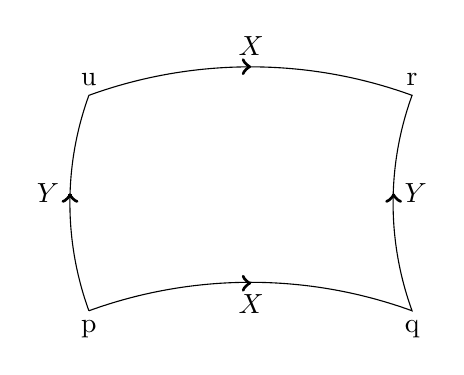
\begin{tikzpicture}
        \draw (0,0) 
            node[below] {p} arc (200:160:4)
            node[above] {u} arc (110:70:6)
            node[above] {r} arc (160:200:4)
            node[below] {q} arc (70:110:6);
            \draw[very thick,->] (-0.24,1.48) -- (-0.24,1.49) node[left] {\(Y\)};
            \draw[very thick,->] (3.87,1.48) -- (3.87,1.49) node[right] {\(Y\)};
            \draw[very thick,->] (2.05,0.35) -- (2.06,0.35) node[below] {\(X\)};
            \draw[very thick,->] (2.05,3.1) -- (2.06,3.1) node[above] {\(X\)};
    \end{tikzpicture}
\end{figure}
Let \(Z_p\in\mathcal{T}_p(\mathcal{M})\) be parallely transported along the path described by \(pqrup\) to get \(Z_p'\in\mathcal{T}_p(\mathcal{M})\). It can be shown that
\begin{equation}
    \lim_{\delta s,\delta t\to0} \frac{(Z_p'-Z_p)^a}{\delta s\delta t} = (R\indices{^a_{bcd}}Z^bY^cX^d)_p.
\end{equation}
Thus curvature measures the change of vectors under parallel transport along closed curves. Equivalently: curvature measure the path dependence of parallel transport.

\subsection{Symmetries of the Riemann tensor}
The first symmetry of the Riemann tensor is self-evident from its definition:
\begin{equation}
    R\indices{^a_{bcd}} = - R\indices{^a_{bdc}}
\end{equation}

Now let the connection be torsion-free and let \(p\in\mathcal{M}\) with \((x^\mu)\) normal coordinates at \(p\).

We have \(\Gamma^\mu_{\nu\rho} = 0\) at \(p\), so \(R\indices{^\mu_{\nu\rho\sigma}}=\partial_\rho\Gamma^\mu_{\nu\sigma} - \partial_\sigma\Gamma^\mu_{\nu\rho}\) at \(p\). Antisymmetrising on \(\nu,\rho,\sigma\) and using \(\Gamma^\mu_{\nu\rho}=0\), we have \(R\indices{^\mu_{[\nu\rho\sigma]}} = 0\) at \(p\). This is a tensorial equation, so it holds in all coordinate systems, and hence
\begin{equation}
    R\indices{^a_{[bcd]}} = 0 \;\text{everywhere}.
\end{equation}

We also have \(\nabla_\tau R\indices{^\mu_{[\nu\rho\sigma]}} = \partial_\tau R\indices{^\mu_{\nu\rho\sigma}} = \partial_\tau\partial_\rho\Gamma^\mu_{\nu\sigma} - \partial_\tau\partial_\sigma\Gamma^\mu_{\nu\rho}\) at \(p\). Antisymmetrising on \(\rho,\sigma,\tau\), we obtain
\begin{equation}
    R\indices{^\mu_{\nu[\rho\sigma;\tau]}} = 0 \implies R\indices{^a_{b[cd;e]}}.
\end{equation}
This is the \emph{Bianchi identity}.

\subsection{Geodesic deviation}
Our goal now is to quantify the relative acceleration of geodesics.

\begin{defn}
    Let \((\mathcal{M},\Gamma)\) be a manifold with a connection. A \emph{1-parameter family of geodesics} is a map \(\gamma:I\times I'\to\mathcal{M}\) where \(I,I'\subset\RR\) are open, satisfying:
    \begin{itemize}
        \item For fixed \(s\), \(\gamma(s,t)\) is a geodesic with affine parameter \(t\).
        \item Locally, \((s,t)\mapsto\gamma(s,t)\) is smooth, 1-to-1, and has a smooth inverse.
    \end{itemize}
    The family of geodesics forms a 2-dimensional surface \(\Sigma \subset \mathcal{M}\).
\end{defn}

Let \(T\) be the tangent to \(\gamma(s=\text{constant},t)\) and \(S\) the tangent to \(\gamma(s,t=\text{constant})\). In coordinates \((x^\mu)\), we have \(S^\mu = \pdv{x^\mu}{s}\), so we can write
\begin{equation}
    x^\mu(s+\delta s,t) = x^\mu(s,t) + \delta s S^\mu(s,t) + O(\delta s^2).
\end{equation}
Hence \(\delta s S\) points from one geodesic to a nearby one; it is known as the \emph{deviation vector}.

\begin{defn}
    The \emph{relative velocity} of nearby geodesics is \(\Delta_T(\delta_s S) = \delta_s \nabla_T S\). 

    The \emph{relative acceleration} of nearby geodesics is \(\delta_s \Delta_T \Delta_T S\).
\end{defn}

If there is no torsion, the geodesic deviation equation holds:
\begin{equation}
    \Delta_T \Delta_T S = R(T,S)T
\end{equation}
\begin{proof}
    Use coordinates \((s,t)\) on \(\Sigma\) and extend to coordinates \((s,t,\dots)\) on a neighbourhood of \(\Sigma\). We have \(S=\pdv{s}\), \(T=\pdv{t}\) and \([S,T]=0\). Since there is no torsion, we have
    \begin{equation}
        \nabla_T S -\nabla_S T = [T,S] = 0 \implies \nabla_T \nabla_T S = \nabla_T\nabla_S T = \nabla_S\underbrace{\nabla_T T}_{=0} + R(T,S) T = R(T,S) T.
    \end{equation}
\end{proof}

Iff \(R\indices{^a_{bcd}} = 0\), then relative acceleration vanishes for all families of geodesics.

Tidal forces arise from geodesic deviation.

\subsection{Curvature of the Levi-Civita connection}
From now on, manifolds are assumed to have a metric and the connection is Levi-Civita unless stated otherwise. Note \(R_{abcd} = g_{ae}R\indices{^e_{bcd}}\).

\begin{defn}
    The \emph{Ricci scalar} is \(R = g^{ab}R_{ab}\). The \emph{Einstein tensor} is \(G_{ab} = R_{ab} - \frac12g_{ab}R\).
\end{defn}

\begin{lemma}
    \begin{enumerate}
        \item \(R_{abcd} = R_{cdab}\) (\(\implies R_{bacd} = -R_{abcd}\))
        \item \(R_{ab} = R_{ba}\)
        \item \(\nabla^aG_{ab}=0\) (\emph{contracted Bianchi identity})
    \end{enumerate}
\end{lemma}
\begin{proof}
    \begin{enumerate}
        \item Let \(p\in\mathcal{M}\) and use normal coordinates at \(p\). We have \(\partial_\rho g_{\mu\nu}=0\), so by the chain rule we have
            \begin{equation}
                0 = \partial_\mu\delta_\rho^\nu = \partial_\mu(g^{\nu\sigma}g_{\sigma\rho}) = g_{\sigma\rho}\partial_\mu g^{\nu\sigma} \implies \partial_\mu g^\nu\tau = 0.
            \end{equation}
            Therefore we have
            \begin{equation}
                \partial_\rho \Gamma^\tau_{nu\sigma} = \frac12g^{\tau\mu} (\partial_\rho\partial_\sigma g_{\mu\nu} + \partial_\rho\partial_\nu g_{\sigma\mu} - \partial_\rho\partial_\mu g_{\nu\sigma}),
            \end{equation}
            and so
            \begin{equation}
                R_{\mu\nu\rho\sigma} = \frac12(\partial_\rho\partial_\nu g_{\sigma\mu} + \partial_\sigma\partial_\mu g_{\nu\rho} - \partial_\sigma \partial_\nu g_{\rho\mu} - \partial_\rho\partial_\mu g_{\nu\sigma}) = R_{\rho\sigma\mu\nu}.
            \end{equation}
        \item \(R_{ab} = g^{cd} R_{dacb} = g^{cd} R_{cbda} = R_{ba}\).
        \item This follows from contracting the Bianchi identity and using the above.
    \end{enumerate}
\end{proof}

\subsection{Einstein's equation}

We are now ready to complete the postulates of general relativity. The complete list is as follows:
\begin{enumerate}
    \item Spacetime is a 4-dimensional Lorentzian manifold with a metric and Levi-Civita connection.
    \item Free particles follow timelike or null geodesics.
    \item The energy, momentum and stress of matter are described by a symmetric, conserved tensor \(T_{ab}\).
    \item Curvature is related to matter by the Einstein equations:
        \begin{equation}
            G_{ab} = R_{ab} - \frac12 g_{ab} R = \frac{8\pi G}{c^4} T_{ab}
        \end{equation}
\end{enumerate}
Einstein's first guess was to set \(R_{ab} = \kappa T_{ab}\). Use the contracted Bianchi identity to write
\begin{equation}
    0 = \nabla^b G_{ab} = \nabla^b R_{ab} -\frac12g_{ab}\nabla^b R = \underbrace{\nabla^b T_{ab}}_{=0} - \frac12g_{ab}\nabla^bT.
\end{equation}
So \(\nabla^b T = 0\). But usually \(T=0\) outside of matter and \(T\ne0\) inside of matter, so this fails. 

In a vacuum, \(T_{ab}=0\) and the Einstein equations are \(R_{ab}-\frac12g_{ab}R=0\). Contracting over \(ab\), we get \(-R=0\), so the vacuum Einstein equations can simply be written \(R_{ab} = 0\).

\begin{theorem}[Lovelock]
    Let \(H_{ab}\) be a symmetric \((0,2)\) tensor satisfying:
    \begin{enumerate}
        \item For all charts \(\phi\) we have \(H_{\mu\nu} = H_{\mu\nu}(g_{\mu\nu},\partial_\rho g_{\mu\nu},\partial_\sigma\partial_\rho g_{\mu\nu})\) at all \(p\in \mathcal{M}\).
        \item \(\nabla^b H_{ab}=0\).
        \item \(H_{\mu\nu}\) is linear in \(\partial_\sigma\partial_\rho g_{\mu\nu}\).
    \end{enumerate}
    Then there exist \(\alpha,\beta\in\RR\) such that \(H_{ab} = \alpha G_{ab} + \beta g_{ab}\).
\end{theorem}
This theorem leads to a modification of the Einstein equation to include a \emph{cosmological constant}:
\begin{equation}
    G_{ab} + \Lambda g_{ab} = 8\pi T_{ab}
\end{equation}
We have set \(G=c=1\).

\section{Diffeomorphisms and Lie derivatives}

\subsection{Maps between manifolds}
\begin{defn}
    Let \(\mathcal{M},\mathcal{N}\) be differentiable manifolds of dimension \(m,n\) respectively. A function \(\phi:\mathcal{M}\to\mathcal{N}\) is \emph{smooth} iff \(\psi_A\circ\phi\psi_\alpha^{-1}:\RR^m\to\RR^n\) is smooth for all charts \(\psi_A\) on \(\mathcal{N}\) and \(\psi_\alpha\) on \(\mathcal{M}\).
\end{defn}
\begin{defn}
    Let \(\phi:\mathcal{M}\to\mathcal{N}\), \(f:\mathcal{N}\to\RR\) be smooth. The \emph{pullback} of \(f\) by \(\phi\) is the map \(\phi^*f:\mathcal{M}\to\RR,p\mapsto\phi^*f(p) = f(\phi(p))\).
\end{defn}
\begin{defn}
    The \emph{pushforward} of a curve \(\lambda:I\to\mathcal{M}\) is \(\phi_*\lambda = \phi\circ\lambda:I\to\mathcal{N},t\to\phi(\lambda(t))\).
\end{defn}
\begin{defn}
    Let \(p\in\mathcal{M}\), and let \(X\in\mathcal{T}_p(\mathcal{M})\) be the tangent vector of a curve \(\lambda:I\to\mathcal{M}\). The \emph{pushforward} of \(X\) by \(\phi\) is \(\phi_*X\in\mathcal{T}_{\phi(p)}(\mathcal{N})\), defined as the tangent of \(\phi_*\lambda\) at \(\phi(x)\).
\end{defn}

\begin{lemma}
    Let \(X\in\mathcal{T}_p(\mathcal{M})\) and \(f:\mathcal{N}\to\RR\). Then \((\phi_*X)(f) = X(\phi^*f)\).
\end{lemma}
\begin{proof}
    Let \(\lambda(0) = p\). We have
    \begin{equation}
        \left.(\phi_*X)(f)\right|_{\phi(p)} = \left[\dv{t}(f\circ(\phi\circ\lambda))(t)\right]_{t=0} = \left[\dv{t}((f\circ\phi)\circ\lambda)(t)\right]_{t=0} = X(\phi^*f).
    \end{equation}
\end{proof}

\begin{defn}
    Let \(\phi:\mathcal{M}\to\mathcal{N}\) be smooth, \(p\in\mathcal{M}\) and \(\eta\in\mathcal{T}^*_{\phi(p)}(\mathcal{N})\). The \emph{pullback} of \(\eta\) by \(\phi\) is \(\phi^*\eta\in\mathcal{T}_p^*(\mathcal{M})\), defined by \((\phi^*\eta)(X) = \eta(\phi_* X)\) for all \(X\in\mathcal{T}_p(\mathcal{M})\).
\end{defn}

\begin{lemma}
    Let \(f:\mathcal{N}\to\RR\). The gradient of \(f\) at \(\phi(p)\) is \(\dd{f}\in\mathcal{T}_{\phi(p)}^*(\mathcal{N})\). We have \(\phi^*(\dd{f}) = \dd{(\phi^*f)}\).
\end{lemma}
\begin{proof}
    Let \(X \in \mathcal{T}_p(\mathcal{M})\). Then \((\phi^*(\dd{f}))(X) = \dd{f}(\phi_*X) = (\phi_*X)(f) = X(\phi^*f) = [\dd{(\phi^*f)}](X)\).
\end{proof}

Let \(x^\mu\) be coordinates on \(\mathcal{M}\) and \(y^\alpha\) coordinates on \(\mathcal{N}\). \(\phi:\mathcal{M}\to\mathcal{N}\) defines a map \(x^\mu\mapsto y^\alpha(x^\mu)\). One can show that for a vector \(X\in\mathcal{T}_p(\mathcal{M})\) we have
\begin{equation}
    (\phi_*X)^\alpha = \left.\pdv{y^\alpha}{x^\mu}\right|_pX^\mu,
\end{equation}
and for a 1-form \(\eta\in\mathcal{T}_P^*(\mathcal{N})\) we have
\begin{equation}
    (\phi^*\eta)_\mu = \left.\pdv{y^\alpha}{x^\mu}\right|_p\eta_\alpha.
\end{equation}

Note that we have not required that \(\phi\) is invertible, so we only have:
\begin{table}[H]
    \centering
    \begin{tabular}{ccc}
        \toprule
                    & pushforward & pullback \\
        \midrule
        functions   & \xmark      & \cmark \\
        curves      & \cmark      & \xmark \\
        vectors     & \cmark      & \xmark \\
        1-forms     & \xmark      & \cmark \\
        \bottomrule
    \end{tabular}
\end{table}

\(p\in\mathcal{M}\) was arbitrary, so the pushforward similarly applies to vector fields and the pullback to covector fields.

We can define the pullback of a \((0,s)\) tensor \(S\) by
\begin{equation}
    (\phi^*S)(X_1,\dots,X_s) = S(\phi_*(X_1),\dots,\phi_*(X_s)) \qq{for all} X_1,\dots,X_s \in \mathcal{T}_p(\mathcal{M}).
\end{equation}
Similarly we can define the pushforward of a \((r,0)\) tensor \(T\) by
\begin{equation}
    (\phi_*T)(\eta_1,\dots,\eta_r) = T(\phi^*\eta_1,\dots,\phi^*\eta_r) \qq{for all} \eta_1,\dots,\eta_r \in \mathcal{T}_p^*(\mathcal{M}).
\end{equation}
These have components given by
\begin{align}
    (\phi^*S)_{\mu_1\dots\mu_s} &= \left.\pdv{y^{\alpha_1}}{x^{\mu_1}}\right|_p\dots\left.\pdv{y^{\alpha_s}}{x^{\mu_s}}\right|_p S_{\alpha_1\dots\alpha_s}, \\
    (\phi_*T)^{\alpha_1\dots\alpha_r} &= \left.\pdv{y^{\alpha_1}}{x^{\mu_1}}\right|_p\dots\left.\pdv{y^{\alpha_r}}{x^{\mu_r}}\right|_p S^{\mu_1\dots\mu_r}.
\end{align}

\begin{eg}
    Let \(\mathcal{M} = S^2\), \(\mathcal{N} = \RR^3\). Use \((\theta,\phi)\) spherical coordinates on \(S^2\) and let \(\phi:\mathcal{M}\to\mathcal{N},p(\theta,\phi)\mapsto y^\alpha = (\sin\theta\cos\phi,\sin\theta\sin\phi,\cos\theta)\). Let \(g\) be a Euclidean metric on \(\RR^3\). \(g_{\alpha\beta} = \delta_{\alpha\beta}\) in cartesian coordinates, and the pullback of \(g\) onto \(S^2\) is \((\phi^*g)_{\mu\nu} = \operatorname{diag}(1,\sin^2\theta)\).
\end{eg}

\subsection{Diffeomorphisms and diffeomorphism invariance}

\begin{defn}
    A map \(\phi:\mathcal{M}\to\mathcal{N}\) is a \emph{diffeomorphism} if \(\phi\) is 1-to-1, onto, smooth, and has a smooth inverse. \(\mathcal{M}\) and \(\mathcal{N}\) must have the same dimension.
\end{defn}

\begin{defn}
    Let \(\phi:\mathcal{M}\to\mathcal{N}\) be a diffemorphism and \(T\) a \((r,s)\) tensor on \(\mathcal{M}\). The \emph{pushforward} of \(T\) under \(\phi\) is the \((r,s)\) tensor on \(\mathcal{N}\) given by
    \begin{equation}
        \phi_*T(\eta_1,\dots,\eta_r,X_1,\dots,X_s) = T(\phi^*\eta_1,\dots,\phi^*\eta_r,(\phi^{-1})_*X_1,\dots,(\phi^{-1})_*X_s) 
    \end{equation}
    for all \(\eta_i\in\mathcal{T}_{\phi(p)}^*(\mathcal{N})\) and \(X_i\in\mathcal{T}_{\phi(p)}(\mathcal{N})\). The \emph{pullback} of \(S\) an \((r,s)\) tensor on \(\mathcal{N}\) is defined to be \(\phi^*S = (\phi^{-1})_*S\).
\end{defn}
One can show that the pushforward and pullback commute with contraction and the outer product, and also that the components of the resulting tensor in a coordinate basis are exactly what one would expect from a coordinate change.

There are two viewpoints we can take here. The active viewpoint is that \(\phi:p\mapsto\phi(p)\) is a map between two distinct manifolds. The passive viewpoint is that we are pulling back coordinates \(y^\mu\) from \(\mathcal{N}\) to \(\mathcal{M}\), and so simply have two coordinate charts \(x^\mu,y^\alpha\) on \(\mathcal{M}\).

\begin{defn}
    Let \(\phi:\mathcal{M}\to\mathcal{N}\) be a diffeomorphism, \(\nabla\) a covariant derivative on \(\mathcal{M}\), \(X\) a vector field and \(T\) a tensor on \(\mathcal{N}\). The \emph{pushforward} of \(\nabla\) is the covariant derivative \(\tilde\nabla\) on \(\mathcal{N}\) defined by
    \begin{equation}
        \tilde\nabla_X T = \phi_*[\nabla_{\phi^*X}(\phi^*T)].
    \end{equation}
\end{defn}
One can show:
\begin{itemize}
    \item \(\tilde\nabla\) satisfied the properties of a covariant derivative.
    \item The Riemann tensor of \(\tilde\nabla\) is the pushforward of the Riemann tensor of \(\nabla\).
    \item If \(\nabla\) is the covariant derivative of the Levi-Civita connection of \(g\) on \(\mathcal{M}\), then \(\tilde\nabla\) is the covariant derivative of the Levi-Civita connection of \(\phi_*g\) on \(\mathcal{N}\).
\end{itemize}

We defined a spacetime as a pair \((\mathcal{M},g)\). Now let's add matter fields \(F,\dots\). Two models \((\mathcal{M},g,F,\dots)\) and \((\mathcal{M}',g',F',\dots)\) are taken to be equivalent if there exists a diffeomorphism \(\phi:\mathcal{M}\to\mathcal{M}'\) which carries \(g,F,\dots\) to \(g',F',\dots\), i.e.\ \(g' = \phi_*g\), \(F' = \phi_*F\), \(\dots\). We have active-passive equivalence, so we can say that the models just differ by a coordinate transformation. Hence a spacetime is really an equivalence class of equivalent \((\mathcal{M},g,F,\dots)\). As a consequence, the Einstein equations will not determine all 10 metric components. Physical statements in general relativity must be diffeomorphism invariant -- this is the gauge freedom of general relativity.

\begin{eg}
    The statement ``two geodesics intersect at \(x^\mu = (\dots)\)'' is \emph{not} gauge invariant.
    Consider however a geodesic intersected exactly once by each of two other geodesics. The proper time between the intersections \emph{is} gauge invariant.
\end{eg}

\subsection{Lie derivatives, symmetries}
Pushforwards and pullbacks enable us to compare tensors at different \(p,q \in \mathcal{M}\).
\begin{defn}
    A diffeomorphism \(\phi:\mathcal{M}\to\mathcal{M}\) is a \emph{symmetry transformation} of a tensor field \(T\) if \(\phi_*T=T\) everywhere. An \emph{isometry} is a symmetry transformation of the metric.
\end{defn}

\begin{defn}
    Let \(X\) be a vector field on a manifold \(\mathcal{M}\). Define \(\phi_t:\mathcal{M}\to\mathcal{M}, p\mapsto q = \) a point a parameter distance \(t\) along the integral curve of \(X\) through \(p\). 
\end{defn}
For small enough \(t\), \(\phi_t\) can be shown to be a diffeomorphism.
\(\phi_0\) is the identity, and we have \(\phi_s\circ\phi_t=\phi_{s+t}\), \(\phi_{-t} = (\phi_t)^{-1}\).
If \(\phi_t\) is a diffeomorphism for all \(t\in\RR\), then we can define for all \(p\in\mathcal{M}\) the curve \(\lambda_p:\RR\to\mathcal{M}, t\mapsto\phi_t(p)\).

\begin{defn}
    The \emph{Lie derivative} of a tensor \(T\) along a vector field \(X\) at \(p\in\mathcal{M}\) is 
    \begin{equation}
        (\mathcal{L}_XT)_p = \lim_{t\to0} \frac{[(\phi_{-t})_*T]_p - T_p}{t}.
    \end{equation}
\end{defn}
\(\mathcal{L}_X\) maps \((r,s)\) tensor fields to \((r,s)\) tensor fields. If \(\alpha\) and \(\beta\) are constants, then we have \(\mathcal{L}_X(\alpha S + \beta T) = \alpha\mathcal{L}_XS + \beta\mathcal{L}_XT\).

\begin{defn}
    Let \(\Sigma\) be a \((n-1)\)-dimensional hypersurface in \(\mathcal{M}\), and \(X\) be a vector field that is nowhere tangent to \(\Sigma\). Let \(x^i\), \(i=1,\dots,n-1\), be coordinates on \(\Sigma\). Assign to \(q\in\mathcal{M}\) coordinates \((t,x^i)\) such that \(q\) is a parameter distance \(t\) along the integral curve of \(X\) through \(x^i\) on \(\Sigma\). For sufficiently small \(t\), \((t,x^i)\) is a coordinate chart; these are \emph{adapted coordinates}.
\end{defn}
Note that integral curves of \(X\) have fixed \(x^i\) and parameter \(t\), so we can write \(X=\pdv{t}\). The diffeomorphism \(\phi_t\) sends points \(p\) with \(x^\mu = (t_p,x^i)\) to \(q\) with \(y^\mu = (t_p+t,x^i)\), and we have \(\pdv{y^\mu}{x^\nu} = \delta^\mu_\nu\). Now consider an \((r,s)\) tensor \(T\) in these coordinates. We have
\begin{equation}
    [((\phi_t)_*T)\indices{^{\mu\dots}_{\nu\dots}}]_{\phi_t(p)} = \pdv{y^\mu}{x^\rho}\dots\pdv{y^\sigma}{x^\nu}\dots[T\indices{^{\rho\dots}_{\sigma\dots}}]_p = [T\indices{^{\mu\dots}_{\nu\dots}}]_p.
\end{equation}
Hence
\begin{equation}
    [((\phi_{\pm t})_*T)\indices{^{\mu\dots}_{\nu\dots}}]_p = [T\indices{^{\mu\dots}_{\nu\dots}}]_{\phi_{\mp t}(p)},
\end{equation}
and so at \(p\) with \((t_p,x^i)\), in this chart we have
\begin{equation}
    (\mathcal{L}_XT)\indices{^{\mu\dots}_{\nu\dots}} = \lim_{t\to0}\frac1t[T\indices{^{\mu\dots}_{\nu\dots}}(t_p+t,x^i)-T\indices{^{\mu\dots}_{\nu\dots}}(t_p,x^i)] = \left.\pdv{t} T\indices{^{\mu\dots}_{\nu\dots}}(t,x^i)\right|_{t_p}.
\end{equation}
It follows that we have a Leibniz rule
\begin{equation}
    \mathcal{L}_X(S\otimes T) = (\mathcal{L}_XS)\otimes T + S\otimes(\mathcal{L}_XT),
\end{equation}
and also that \(\mathcal{L}_X\) commutes with contraction.

We still need a chart independent expression. In this chart, \(\mathcal{L}_Xf = \pdv{t}f\) for functions \(f\). Also, \(X(f) = \pdv{t}f\). Thus in any basis we have
\begin{equation}
    \mathcal{L}_Xf = X(f).
\end{equation}
In our chart, \((\mathcal{L}_XY)^\mu = \pdv{Y^\mu}{t}\) for a vector field \(Y\). Also, since \(X^\mu = \delta_0^\mu\), we have \([X,Y]^\mu = \pdv{Y^\mu}{t}\). Hence in any basis we have
\begin{equation}
    \mathcal{L}_XY = [X,Y].
\end{equation}
Note that \(\mathcal{L}_XT\) depends on \(X_p\) and its derivatives, so neither \(\mathcal{L}\) nor \(\mathcal{L}T\) are tensors. Compare this with covariant derivatives, where \(\nabla_XT\) only depends on \(X_p\), so \(\nabla T\) is a tensor.

One can show:
\begin{itemize}
    \item For a 1-form \(\omega\), we have \((\mathcal{L}_X\omega)_\mu = X^\nu\partial_\nu \omega_\mu + \omega_\nu\partial_\mu X^\nu\), so
        \begin{equation}
            (\mathcal{L}_X\omega)_a = X^b\nabla_b\omega_a + \omega_b\nabla_a X^b.
        \end{equation}
    \item For \ tensor \(T\), we have
        \begin{equation}
            (\mathcal{L}_XT)\indices{^{\alpha\dots}_{\beta\dots}} = X^\gamma\partial_\gamma T\indices{^{\alpha\dots}_{\beta\dots}} - (\partial_\gamma X^\alpha) T\indices{^{\gamma\dots}_{\beta\dots}} - \dots + (\partial_\beta X^\gamma) T\indices{^{\alpha\dots}_{\gamma\dots}} + \dots,
        \end{equation}
        so 
        \begin{equation}
            (\mathcal{L}_X T)\indices{^{a\dots}_{b\dots}} = X^c\nabla_c T\indices{^{a\dots}_{b\dots}} - (\nabla_c X^a)T\indices{^{c\dots}_{b\dots}} - \dots + (\nabla_b X^c)T\indices{^{a\dots}_{x\dots}} + \dots.
        \end{equation}
\end{itemize}

In particular, for the metric, we have
\begin{align}
    (\mathcal{L}_Xg)_{\mu\nu} &= X^\rho\partial_\rho g_{\mu\nu} + g_{\mu\rho}\partial_\nu X^\rho + g_{\rho\nu}\partial_\mu X^\rho \\
                              &= g_{\mu\rho}\nabla_\nu X^\rho + g_{\rho\nu}\nabla_\mu X^\rho \\
                              &= \nabla_\nu X_\mu + \nabla_\mu X_\nu \quad (\text{for Levi-Civita connection}).
\end{align}
Let \(\phi_t\) be a continuous family of isometries. For all \(t\in\RR\) we have \((\phi_t)_*g = g\) and hence \(\mathcal{L}_X(g) = 0\), so using the above we obtain 
\begin{equation}
    \nabla_a X_b + \nabla_b X_a = 0;
\end{equation}
this is \emph{Killing's equation}. Solutions to Killing's equation are called \emph{Killing vector fields}.

If there exists a chart with one coordinate \(z\) on which \(g_{\mu\nu}\) does not depend, then \(\pdv{z}\) is a Killing vector field. Conversely if there is a Killing vector field, then we can choose coordinates such that \(g_{\mu\nu}\) does not depend on one of them.

\begin{lemma}
    Let \(X\) be a Killing vector field, and let \(V\) be a a vector field tangent to an affinely parametrised geodesic. Then \(X_aV^a\) is constant along the geodesic.
\end{lemma}
\begin{proof}
    \begin{align}
        \dv{\tau}(X_aV^a) &= V(X_a V^a) = \nabla_V(X_a V^a) = V^b\nabla_b(X_aV^a) \\
                          &= \underbrace{V^aV^b}_{\mathclap{\text{symmetric}}}\overbrace{\nabla_bX_a}^{\mathclap{\text{antisymmetric}}} + X_a \underbrace{V^b\nabla_b B^a}_{=0} \\
                          &= 0
    \end{align}
\end{proof}

One can show that if \(T_{ab}\) is the energy-momentum tensor and \(X^a\) is a Killing vector field, then the current \(J^a = T\indices{^a_b}\) is conserve, i.e.\ \(\nabla_a J^a = 0\).

\section{Linearised Theory}
\subsection{The linearised Einstein equations}

Consider small deviations from Minkowski spacetime in cartesian coordinates. The ``background'' spacetime is the manifold \(\mathcal{M}=\RR^4\) with metric \(g = \eta = \operatorname{diag}(-1,1,1,1)\), and the ``perturbation'' is a small change to the metric given by \(h = O(\epsilon) \ll 1\) so that \(g = \eta + h\). We regard \(h_{\mu\nu}\) as a tensor field on the background spacetime.

We have two metrics, \(\eta_{\mu\nu}\) and \(g_{\mu\nu}\). The inverse of \(g_{\mu\nu}\) is \(g^{\mu\nu} = \eta^{\mu\nu} - h^{\mu\nu}\) to \(O(\epsilon)\). Also to \(O(\epsilon)\), it can be shown that
\begin{equation}
    \Gamma^\mu_\nu\rho = \frac12\eta^{\mu\sigma} (\partial_\rho h_{\sigma\nu} + \partial_\nu h_{\sigma\rho} - \partial_\sigma h_{\nu\rho}) = O(\epsilon).
\end{equation}
Hence we have
\begin{align}
    & R_{\mu\nu\rho\sigma} = \eta_{\mu\tau}(\partial_\rho\Gamma^\tau_{\nu\sigma} - \partial_\sigma\Gamma^\tau_{\nu\rho}) 
    = \frac12(\partial_\rho\partial_\nu h_{\mu\sigma} + \partial_\sigma \partial_\mu h_{\nu\rho} - \partial_\rho\partial_\mu h_{\nu\sigma} - \partial_\nu\partial_\sigma h_{\mu\rho}) \\
    \implies & R_{\mu\nu} = \partial^\rho\partial_{(\mu}h_{\nu)\rho} - \frac12\partial^\rho\partial_\rho h_{\mu\nu} - \frac12\partial_\mu\partial_\nu h \\
    \implies & G_{\mu\nu} = \partial^\rho\partial_{(\mu}h_{\nu)\rho} - \frac12\partial^\rho\partial_\rho h_{\mu\nu} - \frac12\partial_\mu\nu h - \frac12 \eta_{\mu\nu} (\partial^\rho\partial^\sigma h_{\rho\sigma} - \partial^\rho\partial_\rho h) = 8\pi T_\mu\nu \ll 1,
\end{align}
where \(h = h\indices{^\mu_\mu}\) and \(\partial^\mu = g^{\mu\nu}\partial_\nu\).

\begin{defn}
    The \emph{trace-reversed} perturbation is \(\bar{h}_{\mu\nu} = h_{\mu\nu} - \frac12h\eta_{\mu\nu}\).
\end{defn}
Note that \(h_{\mu\nu} = \bar{h}_{\mu\nu} - \frac12\bar{h}|eta_{\mu\nu}\), i.e.\ if we reverse the trace twice we get the original perturbation. Writing the Einstein tensor in terms of the trace-reversed perturbation simplifies the above expression:
\begin{equation}
    G_{\mu\nu} = -\frac12\partial^\rho\partial_\rho \bar{h}_{\mu\nu} + \partial^\rho\partial_{(\mu}\bar{h}_{\nu)\rho} - \frac12\eta_{\mu\nu}\partial^\rho\partial^\sigma \bar{h}_{\rho\sigma}
\end{equation}

Now let \((\mathcal{M},g,T)\) be a spacetime, and \(\phi:\mathcal{M}\to\mathcal{M}'\) a diffemorphism. Then \((\mathcal{M}',\phi_*g,\phi_*T)\) is a physically equivalent spacetime. We want \(\eta_{\mu\nu}\) to remain the background metric, so we consider \(\phi\sim O(\epsilon)\). Consider diffeomorphism \(\phi_t\) defined by integral curves of a vector field \(X\). Then \(t=O(\epsilon)\). Writing \(\zeta^\mu = tX^\mu = O(\epsilon)\), we have for any tensor \(T\)
\begin{align}
    (\phi_{-t})_*(T) &= T + t\mathcal{L}_XT + O(\epsilon^2) \\
                     &= T + \mathcal{L}_\xi T + O(\epsilon^2).
\end{align}
The energy momentum tensor is \(T_{\mu\nu} = O(\epsilon)\), so \(((\phi_{-t})_*T)_{\mu\nu} = T_{\mu\nu} + O(\epsilon^2)\). The metric becomes
\begin{equation}
    (\phi_{-t})_* g = g + \mathcal{L}_\xi g + \dots = \eta + h + \mathcal{L}_\xi\eta + O(\epsilon^2),
\end{equation}
so \(h_{\mu\nu}\) and \(h_{\mu\nu} + (\mathcal{L}_\xi\eta)_{\mu\nu}\) are physically equivalent. Hence we have a gauge symmetry
\begin{align}
    h_{\mu\nu} &\to h_{\mu\nu} + \partial_\mu \xi_\nu + \partial_\nu \xi_\mu \\
    \implies \bar{h}_{\mu\nu} &\to \bar{h}_{\mu\nu} + \partial_\mu \xi_\nu + \partial_\nu \xi_\mu - \eta_{\mu\nu} \partial_\rho \xi^\rho
\end{align}
for \(\xi_\mu = O(\epsilon)\).

Now choose \(\xi_\mu\) such that \(\partial^\nu\partial_\nu\xi_\mu = -\partial^\nu\bar{h}_{\mu\nu}\). Under this gauge transformation, we have \(\partial^\nu \bar{h}_{\mu\nu} \to 0\) (this is the \emph{Lorentz gauge}), and hence we can choose a gauge so that 
\begin{equation}
    G_{\mu\nu} = -\frac12 \partial^\rho\partial_\rho \bar{h}_{\mu\nu}.
\end{equation}
Thus we have the linearised Einstein equations
\begin{equation}
    \partial^\rho\partial_\rho\bar{h}_{\mu\nu} = -16\pi T_{\mu\nu}.
\end{equation}

\subsection{Newtonian limit}
Newtonian gravity can be summarised by \(\nabla^2\Phi = 4\pi \rho\), accurate for \(\Phi\sim v^2\sim\epsilon \ll 1\). This implies \(\rho \sim O(\epsilon)\), i.e.\ matter sources are weak. For the energy-momentum tensor, we can write
\begin{align}
    T_{00} &= \rho + O(\epsilon^2), \\
    T_{0i} &\sim T_{00} v_i \sim O(\epsilon^{3/2}), \\
    T_{ij} &\sim T_{00}v_iv_j\sim O(\epsilon^2).
\end{align}

For example in a perfect fluid with \(T_{\mu\nu} = (\rho+P)u_\mu u_\nu + P g_{\mu\nu}\), we have \(P\sim \rho \frac{v^2}{c^2}\), and we have \(\frac{P}{\rho}\approx 10^{-5}\) in the sun. In special relativity we have
\begin{equation}
    u^\mu = \left( \frac1{\sqrt{1-v^2}},\frac{v^i}{\sqrt{1-v^2}}\right),
\end{equation}
where \(v^2 = v^iv_i\).

In Newtonian gravity, temporal changes in \(\Phi\) are caused by the motion of sources. Hence we have \(\pdv{t}\sim v\pdv{x^i} = O(\epsilon^{1/2}) \pdv{x^i}\). Therefore \(\dalembertian\,\bar{h}_{\mu\nu} = \partial^\rho\partial_\rho \bar{h}_{\mu\nu} = \partial^i\partial_i\bar{h}_{\mu\nu} = \nabla^2\bar{h}_{\mu\nu} = -16\pi T_{\mu\nu}\), from which we deduce that \(\nabla^2\bar{h}_{00} = -16\pi\rho\), \(\bar{h}_{0i} = O(\epsilon^{3/2})\) and \(\bar{h}_{ij} = O(\epsilon^2)\). The \(00\) component is just Newton's law with \(\bar{h}_{00} = -4\Phi\). Thus we have \(\bar{h} = \eta^{\mu\nu}\bar{h}_{\mu\nu} = 4\Phi = -h\), and so 
\begin{equation}
    h_{00} = \bar{h}_{00} - \frac12\eta_{00}\bar{h} = -2\Phi \qq{and} h_{ij} = -2\Phi\delta_{ij}.
\end{equation}
So in the Newtonian limit, the line element is just
\begin{equation}
    \dd{s}^2 = -(1+2\phi)\dd{t}^2 + (1-2\phi)(\dd{x}^2+\dd{y}^2+\dd{z}^2).
\end{equation}

Now consider geodesics in the weak field. We have Lagrangian
\begin{equation}
    L = -g_{\mu\nu} \dv{x^\mu}{\tau} \dv{x^\nu}{\tau} = (1+2\Phi) \dot{t}^2 - \delta_{ij}(1-2\Phi)\dot{x}^i\dot{x}^j = 1.
\end{equation}
Solving for \(\dot{t}\) we have
\begin{equation}
    \dot{t} = (1-\Phi) + \frac12\delta_{ij}\dot{x}^i\dot{x}^j + O(\epsilon^2).
\end{equation}
The Euler-Lagrance equation for \(x^k\) gives
\begin{equation}
    -2\delta_{jk}\ddot{x}^j + O(\epsilon)^2 = 2\delta_k\Phi.
\end{equation}
Combining these two, we get
\begin{equation}
    \dv[2]{x^k}{t} = \dv[2]{x^k}{\tau} = -\partial_k\Phi,
\end{equation}
i.e.\ the equation of motion for a test body in Newtonian theory.

\subsection{Gravitational waves}

Consider againthe weak field but now in a vacuum, and without the restriction \(\partial_t \ll \partial_i\). The vacuum linearised Einstein equations read
\begin{equation}
    \dalembertian\,\bar{h}_{\mu\nu} = (\partial_t^2 - \nabla^2)\bar{h}_{\mu\nu} = 0.
\end{equation}
This is just a wave equation, and we have the plane wave solution \(\bar{h}_{\mu\nu} = H_{\mu\nu}e^{ik_\mu x^\mu}\), where \(H_{\mu\nu}\) and \(k_\mu\) are constants. \(\dalembertian\,\bar{h}_{\mu\nu} = 0 \implies k_\mu k^\mu = 0\), so the wave propagates at the speed of light. In the Lorentz gauge, \(\partial^\nu\bar{h}_{\mu\nu} = 0 \implies k^\mu H_{\mu\nu} = 0\), i.e.\ oscillations are transverse to the direction of the wave. For example if the wave is in the \(z\)-direction with \(k^\mu = \omega(1,0,0,1)\), then we must have \(H_{\mu0} + H_{\mu3} = 0\).

Note that in the Lorentz gauge we have some remaining gauge freedom to fix. If we take \(\xi_\mu = X_\mu e^{ik_\rho x^\rho}\), then the Lorentz condition is maintained. Under this transformation we have
\begin{equation}
    H_{\mu\nu} \to H_{\mu\nu} + i(k_\mu X_\nu + k_\nu X_\mu - \eta_{\mu\nu} k^\rho X_\rho),
\end{equation}
and from this it can be shown that there is a choice of \(X\) such that \(H_{0\mu} = 0\) and \(H\indices{^\mu_\mu} = 0\). In this gauge, \(h = 0 \implies h_{\mu\nu} = \bar{h}_{\mu\nu}\). For a plane wave in the \(z\)-direction we have \(H_{0\mu} = H_{3\mu} = H\indices{^\mu_\mu} = 0\), so we can write
\begin{equation}
    H_{\mu\nu} = 
    \begin{pmatrix}
        0 & 0 & 0 & 0 \\
        0 & H_+ & H_\times & 0 \\
        0 & H_\times & - H_+ & 0 \\
        0 & 0 & 0 & 0
    \end{pmatrix}
\end{equation}
for constants \(H_+\) and \(H_\times\).

Now consider the effect this wave has on particles. Consider a particle at rest in the background frame with 4-velocity \(u^\alpha(0) = (1,0,0,0)\). The geodesic equation is
\begin{equation}
    \dv{t}u^\alpha + \underbrace{\Gamma^\alpha_{\mu\nu}}_{O(\epsilon)} u^\mu u^\nu = \dot{u}^\alpha + \Gamma^\alpha_{00} = 0.
\end{equation}
Since \(H_{0\mu} = 0\), we have \(\Gamma^\alpha_{00} = \frac12\eta^{\alpha\beta} (\partial_0 h_{\beta0} + \partial_0 h_{0\beta} - \partial_\beta h_{00}) = 0\). Hence \(u^\alpha(\tau) = (1,0,0,0)\), and the particle stays at \(x^i = \text{constant}\) in this gauge. We are interested in proper separations between particles, so we must use the metric, which is
\begin{equation}
    \dd{s}^2 = -\dd{t}^2 + (1+h_+)\dd{x}^2 + (1-h_+)\dd{y}^2 + 2h_\times\dd{x}\dd{y} + \dd{z}^2.
\end{equation}
First consider the case in which \(H_\times = 0\) and \(H_+=0\), so that only \(h_+\) oscillates. The proper separation between 2 particles at \((\pm\delta,0,0)\) is given by \(\dd{s}^2 = (1+h_+)4\delta^2\); similarly for 2 particles at \((0,\pm\delta,0)\) we have \(\dd{s}^2 + (1-h_+)4\delta^2\). Hence the particles move like:
\begin{figure}[H]
    \centering
    \begin{tikzpicture}
        \begin{scope}
            \fill (0.8,0) circle (0.05);
            \fill (-0.8,0) circle (0.05);
            \fill (0,0.8) circle (0.05);
            \fill (0,-0.8) circle (0.05);
        \end{scope}
        \draw[shift={(0,0)},->,very thick] (1.3,0) -- (1.7,0);
        \begin{scope}[shift={(3,0)},xscale=0.6,yscale=1.6]
            \fill (0.8,0) circle (0.05);
            \fill (-0.8,0) circle (0.05);
            \fill (0,0.8) circle (0.05);
            \fill (0,-0.8) circle (0.05);
        \end{scope}
        \draw[shift={(3,0)},->,very thick] (1.3,0) -- (1.7,0);
        \begin{scope}[shift={(6,0)}]
            \fill (0.8,0) circle (0.05);
            \fill (-0.8,0) circle (0.05);
            \fill (0,0.8) circle (0.05);
            \fill (0,-0.8) circle (0.05);
        \end{scope}
        \draw[shift={(6,0)},->,very thick] (1.3,0) -- (1.7,0);
        \begin{scope}[shift={(9.3,0)},xscale=1.6,yscale=0.6]
            \fill (0.8,0) circle (0.05);
            \fill (-0.8,0) circle (0.05);
            \fill (0,0.8) circle (0.05);
            \fill (0,-0.8) circle (0.05);
        \end{scope}
    \end{tikzpicture}
\end{figure}
Now consider \(H_\times \ne 0,H_+=0\). For 2 particles at \((\pm\delta,\pm\delta,0)/\sqrt{2}\) we have \(\dd{s}^2=(1+h_\times)4\delta^2\), and for 2 particles at \((\pm\delta,\mp\delta,0)/\sqrt{2}\) we have \(\dd{s}^2 = (1-h_\times)4\delta^2\), so the particles now move like:
\begin{figure}[H]
    \centering
    \begin{tikzpicture}
        \begin{scope}[rotate=45]
            \fill (0.8,0) circle (0.05);
            \fill (-0.8,0) circle (0.05);
            \fill (0,0.8) circle (0.05);
            \fill (0,-0.8) circle (0.05);
        \end{scope}
        \draw[shift={(0,0)},->,very thick] (1.3,0) -- (1.7,0);
        \begin{scope}[shift={(3,0)},rotate=45,xscale=0.6,yscale=1.6]
            \fill (0.8,0) circle (0.05);
            \fill (-0.8,0) circle (0.05);
            \fill (0,0.8) circle (0.05);
            \fill (0,-0.8) circle (0.05);
        \end{scope}
        \draw[shift={(3,0)},->,very thick] (1.3,0) -- (1.7,0);
        \begin{scope}[shift={(6,0)},rotate=45]
            \fill (0.8,0) circle (0.05);
            \fill (-0.8,0) circle (0.05);
            \fill (0,0.8) circle (0.05);
            \fill (0,-0.8) circle (0.05);
        \end{scope}
        \draw[shift={(6,0)},->,very thick] (1.3,0) -- (1.7,0);
        \begin{scope}[shift={(9,0)},rotate=45,xscale=1.6,yscale=0.6]
            \fill (0.8,0) circle (0.05);
            \fill (-0.8,0) circle (0.05);
            \fill (0,0.8) circle (0.05);
            \fill (0,-0.8) circle (0.05);
        \end{scope}
    \end{tikzpicture}
\end{figure}

\subsection{The field far from the source}
Consider a weak field with matter. The linearised equations are \(\partial_\rho\partial^\rho h_{\mu\nu} = -16\pi T_{\mu\nu}\). By introducing a Green's function, we can invert this to find 
\begin{equation}
    \bar{h}_{\mu\nu}(t,\vb{x}) = 4\int\frac{T_{\mu\nu}(t-|\vb{x}-\vb{y}|,\vb{y})}{|\vb{x}-\vb{y}|}\dd[3]{y}.
\end{equation}
We assume that matter has no compact support inside a radius \(d\), so we can take the integral over \(|\vb{y}| < d\). We assume we are far from the source, so we take \(r=|\vb{x}|\gg d\). Hence we can write
\begin{equation}
    |\vb{x}-\vb{y}| = r - \vu{x}\vdot\vb{y} + O(d/r),
\end{equation}
where \(\vu{x} = \frac{\vb{x}}{r}\). Thus we have
\begin{equation}
    T_{\mu\nu}(t-|\vb{x}-\vb{y}|,\vb{y}) = T_{\mu\nu}(t-r,\vb{y}) - \vu{x}\vdot\vb{y} (\partial_0T_{\mu\nu})(t-r,\vb{y}).
\end{equation}
Assuming \(v\ll c\), we have \(\partial_0 T_{\mu\nu} \sim T_{\mu\nu}\frac{v}{d} \ll \frac{T_{\mu\nu}}{d}\), so to leading order we have
\begin{equation}
    \bar{h}_{\mu\nu}(t,\vb{x}) \approx \frac4r\int T_{\mu\nu}(t-r,\vb{y})\dd[3]{y}.
    \label{invertedlin}
    \tag{\(*\)}
\end{equation}

In the Lorentz gauge, \(\partial^\nu\bar{h}_{\mu\nu} = 0 \implies \partial_0 \bar{h}_{0i} = \partial_j \bar{h}_{ji}\) and \(\partial_0\bar{h}_{00} = \partial_i\bar{h}_{0i}\). Our strategy will be to calculate \(\bar{h}_{ij}\to\bar{h}_{0i}\to\bar{h}_{00}\). We have
\begin{equation}
    \int T^{ij}\dd[3]{y} = \int\underbrace{\partial_k(T^{ik}y^j)}_{\mathclap{\substack{\to0\\(\text{surface term})}}} - (\partial_k T^{ik}) y^j\dd[3]{y} = \int(\partial_0 T^{i0})y^j\dd[3]{y},
\end{equation}
since \(\partial_\mu T^{i\mu} = 0\). Thus we can write
\begin{align}
    \int T^{ij} \dd[3]{y} &= \int T^{(ij)} \dd[3]{y} \\
                     &= \partial_0\int T^{0(i}y^{j)}\dd[3]{y} \\
                     &= \partial_0\int \frac12\underbrace{\partial_k(T^{0k}y^iy^j)}_{\to 0} - \frac12(\partial_k T^{0k})y^i y^j\dd[3]{y} \\
                     &= \frac12 \partial_0\partial_0 \int T^{00}\dd[3]{y},
\end{align}
so \(\bar{h}_{ij} = \frac2r\ddot{I}_{ij}(t-r)\) where
\begin{equation}
    I_{ij}(t-r) = \int T_{00}(t-r,\vb{y})y^iy^j\dd[3]{y}
\end{equation}
is the \emph{quadrupole tensor}.

Next we have
\begin{equation}
    \partial_0 \bar{h}_{0i} = \partial_j \bar{h}_{ji} = \partial_j \left(\frac2r \ddot{I}_{ij}(t-r)\right),
\end{equation}
so integrating once over \(t\), we have
\begin{equation}
    \bar{h}_{0i} = \partial_j\left(\frac2r\dot{I}_{ij}(t-r)\right) + C_i= \underbrace{-2\frac{\hat{x}_j}{r^2}\dot{I}_{ij}}_{\mathclap{=O(1/r^2) \to 0}} - 2\frac{\hat{x}_j}{r}\ddot{I}_{ij} + C_i.
\end{equation}
We set the constant of integration with \eqref{invertedlin}, writing
\begin{equation}
    C_i = \frac4r \int T_{0i}(0,\vb{y})\dd[3]{y} = -\frac4r P_i,
\end{equation}
where \(P_i\) is the ``momentum''. We have
\begin{equation}
    \partial_0P_i(t-r) = -\int\partial_0 T_{0i}\dd[3]{y} = -\int\partial_j T_{ji}\dd[3]{y} = 0,
\end{equation}
so \(P_i\) is conserved at leading order.

Finally, to find \(\bar{h}_{00}\) we use \(\partial_0 \bar{h}_{00} = \partial_i h_{0i}\), which similarly gives
\begin{equation}
    \bar{h}_{00} = \partial_i\left(-\frac{2\hat{x}_j}{r}\dot{I}_{ij}(t-r)\right) + C_0 = 2\frac{\hat{x}_i\hat{x}_j}{r}\ddot{I}_{ij}(t-r) + C_0 + O\left(\frac1{r^2}\right).
\end{equation}
We fix \(C_0\) with
\begin{equation}
    C_0 = \frac4r \int T_{00}(0,\vb{Y})\dd[3]{y} = \frac4r E,
\end{equation}
where \(E\) is the energy. We have
\begin{equation}
    \partial_0 E(t-r) = \partial_0\int T_{00}\dd[3]{y} = \int \partial_i T_{i0} \dd[3]{y} = 0,
\end{equation}
so \(E\) is conserved to leading order.

Note that at higher orders \(E\) and \(P_i\) are not conserved.

\subsection{Energy in gravitational waves}
Consider now 2nd order perturbation theory in the vacuum. The notation we will use is
\begin{equation}
    g_{\mu\nu} = \underbrace{\bar{g}_{\mu\nu}}_{\mathclap{\substack{\text{background}\\\text{(typically \(\eta\))}}}} + \underbrace{\delta^{(1)}g_{\mu\nu}}_{\mathclap{\substack{\text{first}\\\text{order}}}} + \underbrace{\delta^{(2)}g_{\mu\nu}}_{\mathclap{\substack{\text{second}\\\text{order}}}} = \eta_{\mu\nu} + h_{\mu\nu} + h^{(2)}_{\mu\nu}.
\end{equation}
We use this style of notation for all quantities.
To find the inverse to the metric, write
\begin{equation}
    g^{\mu\nu} = \eta^{\mu\nu} + \delta^{(1)}g^{\mu\nu} + \delta^{(2)}g^{\mu\nu}.
\end{equation}
We have
\begin{equation}
    g^{\mu\rho}g_{\rho\nu} = \delta^\mu_\nu + \underbrace{h\indices{^\mu_\nu} + \delta^{(1)}g^{\mu\rho}\eta_{\rho\nu}}_{\text{first order}} + \underbrace{\delta^{(2)}g^{\mu\rho}\eta_{\rho\nu} + h\indices{^{(2)\mu}_\nu} + \delta^{(1)}g^{\mu\rho}h_{\rho\nu}}_{\text{second order}},
\end{equation}
where \(h\indices{^{(2)\mu}_\nu} = \eta^{\mu\rho}h^{(2)}_{\rho\nu}\). Thus we can deduce
\begin{align}
    \delta^{(1)}g^{\mu\nu} &= -h^{\mu\nu} = g^{(1)\mu\nu}[h], \\
    \delta^{(2)}g^{\mu\nu} &= -h^{(2)\mu\nu} + h^{\mu\sigma}h\indices{_\sigma^\nu} = g^{(1)\mu\nu}[h^{(2)}] + g^{(2)\mu\nu}[h].
\end{align}
This is a generic pattern in perturbation theory. Given \(S\indices{^\mu_\nu}\) a function of the metric, we will obtain first and order terms of the form
\begin{align}
    \delta^{(1)}S^{\mu\nu} &= S^{(1)\mu\nu}[h], \\
    \delta^{(2)}S^{\mu\nu} &= S^{(1)\mu\nu}[h^{(2)}] + S^{(2)\mu\nu}[h].
\end{align}
Cosnsider the Einstein equations. We have
\begin{align}
    G_{\mu\nu} &= \bar{G}_{\mu\nu} + \delta^{(1)}G_{\mu\nu} + \delta^{(2)}G_{\mu\nu} \\
               &= 0 + G^{(1)}_{\mu\nu}[h] + G^{(1)}_{\mu\nu}[h^{(2)}] + G^{(2)}_{\mu\nu}[h],
\end{align}
where
\begin{equation}
    G^{(2)}_{\mu\nu}[h] = R^{(2)}_{\mu\nu}[h] - \frac12 R^{(1)}[h]h_{\mu\nu} - \frac12 R^{(2)}[h]\eta_{\mu\nu}.
\end{equation}
As before, since we are in a vacuum, we have \(G^{(1)}_{\mu\nu}[h] = R^{(1)}_{\mu\nu}[h] = 0\). The vacuity also allows us to write \(G^{(1)}_{\mu\nu}[h^{(2)}] = 8\pi t_{\mu\nu}[h]\), where
\begin{equation}
    t_{\mu\nu}[h] = -\frac1{8\pi}G^{(2)}_{\mu\nu}[h] = -\frac1{8\pi}(R^{(2)}_{\mu\nu}[h] - \frac12\eta^{\rho\sigma} R^{(2)}_{\rho\sigma}[h]\eta_{\mu\nu}).
\end{equation}
Consider the contracted Bianchi identities \(g^{\mu\rho}\nabla_\rho g_{\mu\nu} = 0\). At linear order, these give
\begin{equation}
    \partial^\mu G^{(1)}_{\mu\nu}[h] = 0 \implies \partial^\mu G^{(1)}_{\mu\nu}[h^{(2)}] = 0,
\end{equation}
where the implication comes from the fact that the Bianchi identities hold for \(g=\eta+h^{(2)}\). At quadratic order, making use of \(\bar{G}_{\mu\nu} = \delta^{(1)}G_{\mu\nu} = 0\), they give 
\begin{equation}
    \partial^\mu(G^{(2)}_{\mu\nu}[h]) = \partial^\mu t_{\mu\nu} = 0.
\end{equation}
\(t_{\mu\nu}\) is conserved, like the energy-momentum tensor. In fact, we regard \(t_{\mu\nu}\) as the energy-momentum of the gravitational field.

A problem with this is that \(t_{\mu\nu}\) is gauge dependent. There are two ways to get around this. A global solution is to integrate over all space, leading to things like the ADM mass (see the Black Holes course). A local approximation is to use a ``large'' 4-volume \(V\sim a^4\) as follows.

\begin{defn}
    The \emph{average} of a quantity \(X_{\mu\nu}\) with respect to a weight function \(w(x)\) is 
    \begin{equation}
        \expval{X_{\mu\nu}} = \int_V X_{\mu\nu}(x) w(x) \dd[4]{x}.
    \end{equation}
    \(w(x)\) must satisfy \(\int_V w(x)\dd[4]{x}=1\) and \(w(x)\to 0\) smoothly on \(\partial V\).
\end{defn}

We have
\begin{equation}
    \expval{\partial_\rho X_{\mu\nu}} = \int_V(\partial_\rho X_{\mu\nu})w\dd[4]{x} = -\int_V X_{\mu\nu}(\partial_\rho w)\dd[4]{x}.
\end{equation}
Let \(X_{\mu\nu}\) be oscillating with wavelength \(\lambda\), so that \(\partial_\rho X_{\mu\nu} \sim \frac{X_{\mu\nu}}{\lambda}\). We also have \(\partial_\rho w \sim \frac{W}{a}\). If we assume \(a \gg \lambda\), then
\begin{equation}
    \expval{\partial_\rho X_{\mu\nu}}\sim \frac{X_{\mu\nu}}{a} \ll \frac{X_{\mu\nu}}{\lambda} \sim \partial_\rho X_{\mu\nu}.
\end{equation}
Hence we can neglect total derivatives when taking averages. We can do things like \(\expval{A\partial B} = \expval{\partial(AB)} - \expval{(\partial A) B} \approx - \expval{(\partial A)B}\). Using this fact, we find
\begin{equation}
    \expval{\eta^{\mu\nu}R^{(2)}_{\mu\nu}[h]} = 0
\end{equation}
and
\begin{equation}
    \expval{t_{\mu\nu}} = \frac1{32\pi}\expval{\partial_\mu\bar{h}_{\rho\sigma}\partial_\nu\bar{h}^{\rho\sigma} - \frac12\partial_\mu\bar{h}\partial_\nu\bar{h} + 2\partial_\rho\bar{h}^{\rho\sigma}\partial_{(\mu}\bar{h}_{\nu)\sigma}}.
\end{equation}
This expression for \(\expval{t_{\mu\nu}}\) is gauge invariant.

\subsection{Quadrupole formula}
The energy flux in gravitational waves is given by \(-\expval{t_{0i}}\). Consider a sphere far from the source with \(r\gg d\), and let \(\hat{x}_i = \frac{x_i}{r}\). The power through the sphere is given by
\begin{equation}
    \expval{p} = -\int r^2\expval{t_{0i}}\hat{x}^i\dd{\Omega}
\end{equation}
where \(\dd{\Omega} = \sin\theta\dd{\theta}\dd{\phi}\). In the Lorentz gauge \(\partial^\nu\bar{h}_{\nu\rho}=0\), we have
\begin{equation}
    \expval{t_{0i}} = \frac1{32\pi}\expval{\partial_0\bar{h}_{\rho\sigma}\partial_i\bar{h}^{\rho\sigma} - \frac12\partial_0\bar{h}\partial_i\bar{h}}.
\end{equation}
Using the value for \(\bar{h}_{\rho\sigma}\) from before, doing a lot of algebra, and taking things to \(O\left(\frac1r\right)\), we obtain
\begin{equation}
    \expval{p}_t = \frac15\expval{\dddot{Q}_{ij}\dddot{Q}_{ij}}_{t-r} \qq{where} Q_{ij} = I_{ij}-\frac13I_{kk}\delta_{ij}.
\end{equation}
This is the \emph{quadrupole formula}.

\section{Differential Forms}
\subsection{\texorpdfstring{$p$}{p}-forms}

\begin{defn}
    A \emph{\(p\)-form} is a totally antisymmetric tensor of rank \((0,p)\).
\end{defn}
0-forms are functions and 1-forms are covectors.
\begin{defn}
    Let \(\eta\) be a \(p\)-form and \(\omega\) a \(q\)-form. Their wedge product \(\eta\wedge\omega\) is a \((p+q)\)-form defined by
    \begin{equation}
        (\eta\wedge\omega)_{a_1\dots a_pb_1\dots b_q} = \frac{(p+q)!}{p!q!}\eta_{[a_1\dots a_p}\omega_{b_1\dots b_q]} \iff \eta\wedge\omega = \frac{(p+q)!}{p!q!} \mathcal{A}(\eta\otimes\omega),
    \end{equation}
    where \(\mathcal{A}\) is an operator that totally antisymmetrises the given tensor.
\end{defn}
One can show that \(\eta\wedge\omega=(-1)^{pq}\omega\wedge\eta\), so \(\eta\wedge\eta = 0\) if \(p\) is odd. Also, the wedge product is associative:
\begin{equation}
    (\eta\wedge\omega)\wedge\chi = \eta\wedge(\omega\wedge\chi)
\end{equation}

Given a dual basis \(\{f^\mu\}\), the \(p\)-forms
\begin{equation}
    f^{\mu_1}\wedge\dots\wedge f^{\mu_p} = p!(f^{[\mu_1}\otimes\dots\otimes f^{\mu_p]})
\end{equation}
form a basis for the space of \(p\)-forms. We will often expand a \(p\)-form in terms of its components in this basis as
\begin{equation}
    \eta = \frac1{p!}\eta_{\mu_1\dots\mu_p} f^{\mu_1}\wedge\dots\wedge f^{\mu_p}.
\end{equation}
\begin{defn}
    The \emph{exterior derivative} of a \(p\)-form \(\eta\) is a \((p+1)\)-form \(\dd{\eta}\) given by
    \begin{equation}
        (\dd{\eta})_{\mu_1\dots\mu_{p+1}} = (p+1)\partial_{(\mu_1)}\eta_{\mu_2\dots\mu_{p+1}]} = (p+1)\big[\nabla_{[\mu_1}\eta_{\mu_2\dots\mu_{p+1}} + \underbrace{\Gamma^\rho_{[\mu_2\mu_1}}_{\mathclap{\substack{=0\\\text{(torsion free)}}}}\eta_{|\rho|\mu_3\dots\mu_{p+1}}\big]
    \end{equation}
\end{defn}
It can be shown that:
\begin{itemize}
    \item \(\dd{(\dd{\eta})} = 0\).
    \item \(\dd{(\eta\wedge\omega)} = \dd{\eta}\wedge\omega + (-1)^p\eta\wedge\dd{\omega}\) (\(\eta\) a \(p\)-form).
    \item \(\dd{(\phi^*\eta)} = \phi^*\dd{\eta}\).
\end{itemize}
\begin{defn}
    A \(p\)-form \(\eta\) is \emph{closed} if \(\dd{\eta}=0\), and \emph{exact} if there exists a \((p-1)\)-form \(\omega\) such that \(\eta = \dd{\omega}\).
\end{defn}
Note that if \(\eta\) is exact, then it is closed. The converse is not always true, but we do have:
\begin{lemma}[Poincar\'e lemma]
    If \(\eta\) is closed, then for all points \(r \in \mathcal{M}\) there exists a neighbourhood \(\mathcal{O}\) of \(r\) and a \((p-1)\)-form \(\omega\) such that \(\eta = \dd{\omega}\) in \(\mathcal{O}\).
\end{lemma}
In other words, if \(\eta\) is closed, then it is locally exact.
\subsection{Integration}
\begin{lemma}
    Let \(\omega\) be a \(n\)-form and \(\{f^\mu\}\) a dual basis for an \(n\)-dimensional manifold \(\mathcal{M}\). Then there exists a function \(h\) such that \(\omega = hf^1\wedge\dots f^n\).
\end{lemma}
\begin{defn}
    An \emph{orientation} of an \(n\)-dimensional manifold \(\mathcal{N}\) is a smooth nowhere vanishing \(n\)-form \(\eta\), up to an equivalence given by \(\eta\sim\eta'\) iff there exists a function \(h>0\) such that \(\eta' = h\eta\).
\end{defn}
\begin{defn}
    A coordinate chart \(x^\mu\) on \(\mathcal{N}\) is \emph{right-handed} relative to a given orientation \(\eta\) if there exists a function \(h>0\) such that \(\eta = h\dd{x^1}\wedge\dots\wedge\dd{x^\mu}\).
\end{defn}
\begin{defn}
    The \emph{volume form} on \((\mathcal{N},g)\) is \(\varepsilon = \sqrt{|g|}f^1\wedge\dots\wedge f^n\), where \(g=\det{g_{\alpha\beta}}\).
\end{defn}
\begin{defn}
    Let \(\psi = x^\mu:\mathcal{O}\subset\mathcal{N}\to\RR^n\) be a right-handed coordinate chart, and \(\omega\) a \(n\)-form. Then the integral of \(\omega\) over \(\mathcal{O}\) is
    \begin{equation}
        \int_{\mathcal{O}}\omega = \int_{\psi(\mathcal{O})\subset\RR^n}\omega_{1\dots n} \dd{x^1}\dots\dd{x^n}.
    \end{equation}
    To integrate over regions with more than one chart, we add these expressions patchwise.
\end{defn}
This expression for the integral can be shown to be chart independent. We can integrate a function \(f\) using the volume form:
\begin{equation}
    \int_{\mathcal{O}} f\varepsilon = \int_{\psi(\mathcal{O})}f\sqrt{|g|}\dd{x^1}\dots\dd{x^n}
\end{equation}
\begin{defn}
    A diffeomorphism \(\phi:\mathcal{N}\to\mathcal{N}\) is \emph{orientation preserving} if \(\phi^*\eta\) is equivalent to \(\eta\) for all orientations \(\eta\).
\end{defn}
If \(\phi\) is orientation preserving, it can be shown that \(\int_{\mathcal{N}}\phi^*\omega=\int_{\mathcal{N}}\omega\).

\subsection{Submanifolds, Stokes' theorem}
Let \(\mathcal{M},\mathcal{N}\) be orientable manifolds of dimensions \(m<n\).
\begin{defn}
    An \emph{embedding} \(\phi:\mathcal{M}\to\mathcal{N}\) is a smooth, 1-to-1 map such that for all \(p\in\mathcal{M}\) there exists a neighbourhood \(\mathcal{O}\) such that \(\phi^{-1}:\phi(\mathcal{O})\to\mathcal{M}\) is smooth. If \(m=n-1\), then \(\phi(\mathcal{M})\) is a \emph{hypersurface}.
\end{defn}
\begin{defn}
    Let \(\phi[\mathcal{M}]\) be \(m\)-dimensional, and let \(\eta\) be an \(m\)-form on \(\mathcal{N}\). Then we define the integral of \(\eta\) over \(\phi[\mathcal{M}]\) as
    \begin{equation}
        \int_{\phi[\mathcal{M}]}\eta = \int_{\mathcal{M}}\phi^*\eta.
    \end{equation}
\end{defn}
Note that if \(\eta = \dd{\omega}\) then we have
\begin{equation}
    \int_{\phi[\mathcal{M}]}\dd{\omega} = \int_{\mathcal{M}}\dd{\phi^*\eta}.
\end{equation}
\begin{defn}
    Let \(\frac12\RR^n=\{(x^1,\dots,x^n)\in\RR\st x^1\le0\}\). A \emph{manifold with boundary} \(\mathcal{N}\) is identical to a manifold, except for that the charts now map to \(\frac12\RR^n\). Its \emph{boundary} is \(\partial\mathcal{N}=\{p\in\mathcal{N} \st x^1(p) = 0\}\), and is \((n-1)\)-dimensional. \((x^2,\dots,x^n)\) is \emph{right-handed} on \(\partial\mathcal{N}\) if \((x^1,\dots,x^n)\) is right-handed on \(\partial\mathcal{M}\).
\end{defn}

\begin{theorem}[Stokes' theorem]
    Given an \(n\)-dimensional orientable manifold \(\mathcal{N}\) with boundary \(\partial\mathcal{N}\) and \((n-1)\)-form \(\eta\), we have
    \begin{equation}
        \int_{\mathcal{N}} \dd{\eta} = \int_{\partial\mathcal{N}} \eta.
    \end{equation}
\end{theorem}

\begin{defn}
    \(X\in\mathcal{T}_p(\mathcal{N})\) is \emph{tangent} to \(\phi(\mathcal{M})\) if there exists a curve in \(\phi(\mathcal{M})\) with tangent \(X\). \(\tilde{n}\in\mathcal{T}_p^*(\mathcal{N})\) is \emph{normal} to \(\phi(\mathcal{M})\) if \(\tilde{n}(X) = 0\) for all \(X\) tangent to \(\phi(\mathcal{M}\).
\end{defn}

\begin{defn}
    Let \(\Sigma\) be a hypersurface of a Lorentzian manifold with normal field \(\tilde{n}\). \(\Sigma\) is \emph{spacelike} (\emph{timelike}, \emph{null}) if \(\tilde{n}\) is \emph{timelike} (\emph{spacelike}, \emph{null}). On \(\partial\mathcal{N}\), \(\dd{x^1}\) is the \emph{outgoing} normal to \(\partial\mathcal{N}\).
\end{defn}

\begin{theorem}[Divergence theorem]
    Let \(\partial\mathcal{N}\) be timelike or spacelike, \(X\) a vector field on \(\mathcal{N}\), and \(h_{\mu\nu} = \phi^*g_{\mu\nu}\) for \(\phi:\partial\mathcal{N}\to\mathcal{N},p\mapsto p\). Then we have
    \begin{equation}
        \int_{\mathcal{N}} \nabla_a X^a\sqrt{|g|} \dd[n]{x} = \int \tilde{n}_a X^a \sqrt{|h|} \dd[n-1]{x}.
    \end{equation}
\end{theorem}

\section{The Initial Value Problem}
\subsection{Extrinsic curvature}
Let \(\mathcal{N}\) be a manifold, \(\Sigma\) a hypersurface, and \(g\) the metric (Riemannian or Lorentzian). The unit normal to \(\Sigma\) is the normal \(n\) such that \(n_an^a = \mp1\). We take the upper sign if \(n\) is timelike, and the lower sign if \(n\) is spacelike.

\begin{defn}
    The \emph{projector} onto \(\Sigma\) is \(\perp\indices{^a_b}=\delta^a_b \pm n^an_b\). Given a tensor \(T\), its \emph{projection} \(\perp T\) onto \(\Sigma\) is given by
    \begin{equation}
        \perp T\indices{^{ab\dots}_{cd\dots}} = \perp\indices{^a_e}\perp\indices{^b_f}\dots\perp\indices{^g_c}\perp\indices{^h_d}\dots T\indices{^{ef\dots}_{gh\dots}}.
    \end{equation}
\end{defn}
We have:
\begin{itemize}
    \item \(\perp\indices{^a_b}n^b=0\) and \(\perp\indices{^a_c}\perp\indices{^c_b} = \perp\indices{^a_b}\), so this is indeed a projection operator.
    \item For all \(X\in\mathcal{T}_p(\mathcal{N})\), we have that \(\perp\indices{^a_b}X^b\) is tangent to \(\Sigma\), and we can write
        \begin{equation}
            X^a = \perp\indices{^a_b}X^b \mp n^an_bX^b.
        \end{equation}
    \item Given \(X,Y\) tangent to \(\Sigma\), we have \(g_{ab} X^aY^b=\perp_{ab}X^aY^a\). For this reason, \(\perp_{ab}\) is often called the \emph{induced metric} on \(\Sigma\), and we write \(\gamma_{ab} = \perp_{ab}\). It is also sometimes called the \emph{1st fundamental form}.
\end{itemize}

Let \(X,Y\) be tangent vector fields to \(\Sigma\), and \(N\) some normal vector field. Parallely transport \(N\) along the integral curves of \(X\) so that \(X^b\nabla_b N^a = 0\). Does \(N\) remain normal to \(\Sigma\)? Not in general. We have
\begin{equation}
    X^b\nabla_b(Y^a N_a) = N_aX^b\nabla_bY^a \ne 0 \;\text{in general}.
\end{equation}
Thus we have another kind of curvature for \(\Sigma\).
\begin{defn}
    Extend the unit normal \(n\) is a neighbourhood of \(\Sigma\), maintaining \(n^an_a = \mp 1\). The \emph{extrinsic curvature} of \(\Sigma\) is the \((0,2)\) tensor 
    \begin{equation}
        \fullfunction{K}{\mathcal{T}_p(\mathcal{N})\times\mathcal{T}_p(\mathcal{N})}{\RR}{X,Y}{n_a(\nabla_{\perp X}(\perp Y))^a}.
    \end{equation}
\end{defn}
Note that we have made a choice of sign convention here.
\begin{lemma}
    \(K_{ab} = -\perp\indices{^c_a}\perp{^d_b}\nabla_c n_d\) and is independent of the extension of \(n\).
\end{lemma}
\begin{proof}
    First we prove the expression. We have
    \begin{align}
        K_{ab}X^aY^b &= n_a(\perp X)^c\nabla_c(\perp Y)^a \\
                     &= -(\perp X)^c(\perp Y)^a\nabla_c n_a \\
                     &= -\perp\indices{^c_b}X^b\perp\indices{^a_d}Y^d\nabla_c n_a \\
        \implies K_{bd} &= -\perp\indices{^c_b}\perp\indices{^a_d}\nabla_c n_a.
    \end{align}
    Now we prove that it is independent of the extension of \(n\). Consider another extension \(n_a'\) and let \(m_a=n_a'-n_a\), which vanishes on \(\Sigma\). On \(\Sigma\), we have
    \begin{align}
        X^a Y^b(K_{ab}-K'_{ab}) &= \perp\indices{^c_a}\perp\indices{^d_b}X^aY^b\nabla_c m_d \\
                                &= (\perp X)^c \big[(\perp Y)^d\nabla_cm_d + \underbrace{m_d}_{\mathclap{=0}}\nabla_c(\perp Y)^d\big]\\
                                &= (\perp X)^c \nabla_c (m_d(\perp Y)^d) = 0.
    \end{align}
\end{proof}
Note that we have \(n^b\nabla_cn^b = \frac12\nabla_c(n_bn^b) = 0\), so we can write
\begin{equation}
    K_{ab} = -\perp\indices{^c_a}\perp\indices{^d_b}\nabla_cn_d = -\perp\indices{^c_a}(\delta^d_b\pm n^dn_b)\nabla_c n_d = -\perp\indices{^c_a}\nabla_c n_b.
\end{equation}
\begin{defn}
    Let \(t:\mathcal{N}\to\RR\) with \(t=\text{constant}\) and \(\dd{t}\ne 0\) on \(\Sigma\). Then we can write the unit normal as \(n = \mp \alpha\dd{t}\), where 
    \begin{equation}
        \alpha = \frac1{\pm\sqrt{g^{-1}(\dd{t},\dd{t})}}
    \end{equation}
    is the \emph{lapse}. The choice of sign means that \(n\) is future pointing if it is timelike.
\end{defn}

\begin{lemma}
    \(K_{ab} = K_{ba}\).
\end{lemma}
\begin{proof}
    We have
    \begin{equation}
        \nabla_cn_d = \mp\nabla_c(\alpha(\dd{t})_d) = \mp \alpha\nabla_c\nabla_d t + (\nabla_c\alpha) \frac{n_d}{\alpha},
    \end{equation}
    so \(K_{ab} = \pm \perp\indices{^c_a}\perp\indices{^d_b}\alpha\nabla_c\nabla_d t\), which is symmetric (for vanishing torsion).
\end{proof}

\begin{defn}
    \(K = K\indices{^b_b} = g^{ab}K_{ab} = \perp^{ab}K_{ab} = \gamma^{ab}K_{ab}\).
\end{defn}

\subsection{The Gauss-Codazzi equations}
\begin{defn}
    The \emph{covariant derivative} \(D_a\) on \(\Sigma\) is defined by
    \begin{equation}
        D_a T\indices{^{b\dots}_{c\dots}} = \perp\indices{^d_a}\perp\indices{^b_e}\dots\perp\indices{^f_c}\dots\nabla_d T\indices{^{e\dots}_{f\dots}}.
    \end{equation}
\end{defn}
It can be shown that \(D\) is torsion free and the Levi-Civita connection of \(\gamma_{ab}\) on \(\Sigma\) if \(\nabla\) is that of \(g_{ab}\) on \(\mathcal{N}\). \(D\) defines the Riemann tensor of \(\gamma_{ab}\), which we write as \(\mathcal{R}\indices{^a_{bcd}}\). One can calculate the projections of \(R\indices{^a_{bcd}}\) using the Ricci identity. We obtain:
\begin{description}
    \item[Gauss equation]: \(\perp R\indices{^a_{bcd}} = \mathcal{R}\indices{^a_{bcd}} \pm 2K\indices{^a_{[c}}K_{d]b}\). 
    \item[Contracted Gauss]: \(\perp R_{ab} \pm \perp\indices{^c_a}n^d\perp\indices{^e_b}n^fR_{cdef} = \mathcal{R}_{ab} \pm KK_{ab}\mp K_{ac}K\indices{^c_b}\).
    \item[Scalar Gauss]: \(R\pm2R_{cd}n^cn^d = \mathcal{R} \pm K^2 \mp K_{cd}K^{cd}\).
    \item[Codazzi]: \(\perp\indices{^d_a}\perp\indices{^e_b}\perp\indices{^f_c}n^gR_{defg} = -D_aK_{bc} + D_bK_{ac}\).
    \item[Contracted Codazzi]: \(\perp\indices{^c_b}R_{cd}n^d = -D_a K\indices{^a_b} + D_bK\).
\end{description}

\subsection{The constraint equations}
From now on we will take \(n\) timelike (so we use the upper sign). We wish to project the Einstein equations \(G_{ab} = 8\pi T_{ab}\) onto \(\Sigma\). From the energy-momentum tensor we define
\begin{equation}
    \rho = R_{ab}n^an^b,\quad j_a = -\perp\indices{^b_a}T_{bc}n^c,\quad S_{ab} = \perp T_{ab}.
\end{equation}
Contracting the Einstein equations with \(n^an^b\), we have \(R_{ab} n^an^b+\frac12 R=8\pi\rho\), and if we substitute in the scalar Gauss equation, we obtain
\begin{equation}
    \mathcal{R}-K_{cd}K^{cd}+K^2-16\pi\rho=0.
\end{equation}
This is the \emph{Hamiltonian constraint}.

If we contract with \(n^a\) and then project with \(\perp\), we get \(\perp\indices{^b_a}n^cR_{bc} = -8\pi j_a\). Substituting in the contracted Codazzi equation, we have
\begin{equation}
    D_cK\indices{^c_a}-D_aK-8\pi j_a = 0.
\end{equation}
This is the \emph{momentum constraint}.

\subsection{Foliations}
\begin{defn}
    A \emph{Cauchy surface} is a spacelike hypersurface \(\Sigma\) in \(\mathcal{N}\) such that each timelike or null curve without endpoints intersects \(\Sigma\) exactly once. \((\mathcal{N},g)\) is \emph{globally hyperbolic} if it admits a Cauchy surface.
\end{defn}
From now on we assume that \((\mathcal{N},g)\) is globally hyperbolic. One can show that this implies that there is a smooth \(\hat{t}:\mathcal{N}\to\RR\) such that \(\dd{\hat{t}}\ne0\) everywhere, and the hypersurfaces \(\Sigma\) are level surfaces with \(\hat{t}=\text{constant}\). Thus for all \(t \in \RR\) we have a surface \(\Sigma_t = \{p\in\mathcal{N}\st \hat{t}(p) = t\}\), and \(\Sigma_t\cap\Sigma_{t'}\ne \varnothing \iff t=t'\). We assume that the \(\Sigma_t\) are spacelike, and that \(\mathcal{N}=\bigcup_{t\in\RR}\Sigma_t\). Such a family of hypersurfaces is called a \emph{foliation} of \(\mathcal{N}\). From now on we will just use \(t\) without referring to \(\hat{t}\).

\begin{defn}
    \(m=\alpha n\) is the \emph{normal evolution vector}.
\end{defn}
Since \(n=-\alpha\dd{t}\) and \(n\vdot n=-1\), we have \(m\vdot m=-\alpha^2\) and \(\expval{\dd{t},m}=-\frac1\alpha\expval{n,m}=1\). Using this we see that \(\mathcal{L}_m t = m(t) = \expval{\dd{t},m} = 1\), so the proper time along integral curves of \(m\) is given by
\begin{equation}
    \tau = \int^t_{t_0}\sqrt{-g(m,m)}\dd{\tilde{t}} \implies \dv{\tau}{t} = \sqrt{-g(m,m)} = \alpha.
\end{equation}
\begin{defn}
    The \emph{acceleration} is \(a_b = n^c\nabla_cn_b\).
\end{defn}
\begin{lemma}
    \(a_b = D_b\log\alpha\).
\end{lemma}
Recall that \(K_{ab} = -\perp\indices{^c_a}\nabla_c n_b = -\nabla_a n_b - n_an^c\nabla_c n_b\), so we can write
\begin{equation}
    \nabla_an_b = -K_{ab}-n_aa_b = -K_{ab}-n_aD_b\log\alpha.
\end{equation}
Hence we have
\begin{equation}
    \nabla_a m_b = \nabla_a(\alpha n_b) = n_b\nabla_a\alpha + \alpha \nabla_a n_b = n_b\nabla_a\alpha - \alpha K_{ab} - n_a D_b \alpha.
\end{equation}
\begin{lemma}
    \begin{itemize}
        \item \(\mathcal{L}_m\gamma_{ab} = -2\alpha K_{ab}\).
        \item \(\mathcal{L}_n\gamma_{ab} = -2K_{ab}\).
        \item \(\mathcal{L}_m\gamma\indices{^a_b} = \mathcal{L}_m\perp\indices{^a_b} = 0\).
        \item \(\mathcal{L}_n\gamma\indices{^a_b} = n^aD_b\log\alpha\).
    \end{itemize}
\end{lemma}
\begin{cor}
    Let \(T\) be a tangent tensor, i.e.\ \(\perp T = T\). Then we have
    \begin{equation}
        \mathcal{L}_m T = \mathcal{L_m}(\perp T) = \underbrace{(\mathcal{L}_m\perp)}_{=0}T + \perp\mathcal{L}_m T = \perp \mathcal{L}_m T,
    \end{equation}
    so \(\mathcal{L}_m T\) is also tangent to \(\Sigma\).
\end{cor}
With these tools we can calculate the final projection. A lot of effort gives
\begin{equation}
    \perp\indices{^e_a}\perp{^g_b}n^hR_{efgh}n^f = \frac1\alpha\mathcal{L}_m K_{ab} + K_{ac}K\indices{^c_b} + \frac1\alpha D_a D_b\alpha.
\end{equation}
With the contracted Gauss equation we have
\begin{equation}
    \perp R_{ab} = -\frac1\alpha\mathcal{L}_mK_{ab} - \frac1\alpha D_aD_b\alpha + \mathcal{R}_{ab} + KK_{ab} - 2K_{ac}K\indices{^c_b}.
\end{equation}
Finally, contracting with \(\perp^{ab}\) and using the scalar Gauss equation, we have
\begin{equation}
    R = \frac2\alpha\mathcal{L}_m K - \frac2\alpha D_cD^c\alpha+\mathcal{R} + K^2 + K_{cd} K^{cd}.
\end{equation}

\subsection{The \texorpdfstring{$3+1$}{3+1} equations}
The Einstein equations can be written as \(R_{ab}=8\pi(T_{ab}-\frac12g_{ab}T)\). Projecting this, we obtain
\begin{equation}
    \perp R_{ab}=4\pi(2S_{ab}+(\rho-S)\gamma_{ab}).
\end{equation}
Using the results of the last section, we find
\begin{equation}
    \mathcal{L}_m K_{ab} = -D_a D_b \alpha + \alpha\left\{R_{ab} + KK_{ab} -2K_{ac}K\indices{^c_b} + 4\pi[(S-\rho)\gamma_{ab}-2S_{ab}]\right\}.
\end{equation}
Now we need to relate \(\mathcal{L}_m\) to a time deriative \(\pdv{t}\). We use adapated coordinates \(x^\alpha = (t,x^i)\), \(i=1,2,3\), where \(x^i\) label points in \(\sigma_t\). This gives a basis \(\partial_t, \partial_i\) and a corresponding dual basis \(\dd{t},\dd{x^i}\). Integral curves of the \(\partial_i\) have \(t=\text{constant}\), so they are in one \(\sigma_t\). What about integral curves of \(\partial_t\)? Clearly \(\expval{\dd{t},\partial_t}=1=\expval{\dd{t},m}\), so \(\expval{\dd{t},\partial_t-m}=0\).
\begin{defn}
    The \emph{shift vector} is \(\beta = \partial_t-m\).
\end{defn}
We have \(\expval{\dd{t},\beta}=0\), and we can write \(\partial_t=\alpha n + \beta\). Curves with \(x^i\) constant are not in general normal to \(\Sigma_t\), and \(\beta\) measures this deviation. 

Using the definitions of \(\alpha\) and \(\beta\), we obtain that the components of the metric are
\begin{equation}
    g_{\alpha\beta} = 
    \begin{pmatrix}
        -\alpha^2+\beta_k\beta^k & \beta_j \\
        \beta_i & \gamma_{ij}
    \end{pmatrix}
    \iff
    g^{\alpha\beta} = 
    \begin{pmatrix}
        -\alpha^{-2} & \alpha^{-2}\beta_j \\
        \alpha^{-2}\beta_i & \gamma^{ij} - \alpha^{-2}\beta^i\beta^j
    \end{pmatrix}.
\end{equation}
Hence we have \(\det g_{\alpha\beta} = -\alpha^2\det\gamma_{ij}\), so \(\sqrt{-g} = \alpha\sqrt{\gamma}\).

In adapted coordinates, the \(3+1\) equations contain only tensors tangent to \(\Sigma_t\), so we can ignore time components and substitute \(i,j,\dots = 1,2,3\) for abstract indices. We have
\begin{equation}
    \mathcal{L}_m\gamma_{ij}=\mathcal{L}_{\partial_t}\gamma_{ij} - \mathcal{L}_\beta\gamma_{ij} = \pdv{t}\gamma_{ij}-\beta^m\partial_m\gamma_{ij} - \gamma_{mj}\partial_i\beta^m - \gamma_{im}\partial_j\beta^m
\end{equation}
and
\begin{equation}
    \mathcal{L}_m K_{ij} = \pdv{t}K_{ij} - \beta^m\partial_m K_{ij} - K_{mj}\partial_i\beta^m - K_{im}\partial_j\beta^j.
\end{equation}
Hence we have:
\begin{align}
    \partial_t \gamma_{ij} &= \mathcal{L}_\beta\gamma_{ij} - 2\alpha K_{ij} \\
    \partial_t K_{ij} &= \mathcal{L}_\beta K_{ij} - D_iD_j\alpha _ \alpha \left\{\mathcal{R}_{ij}+KK_{ij}-2K_{im}K\indices{^m_j} + 4\pi[(S-\rho)\gamma_{ij}-2S_{ij}]\right\}
\end{align}
Together with the constraint equations this is our full set of equations.

Note that \(\alpha,\beta^i\) are freely specifiable, reflecting gauge freedom. Also, it can be shown from the Bianchi identities that the constraints are preserved under time evolution.

\section{The Lagrangian Formulation}

Consider a scalar field in a curved spacetime. The action is
\begin{equation}
    S = \int_{\mathcal{M}} \left[-\frac12g^{\alpha\beta}\nabla_\alpha\phi\nabla_\beta\phi - V(\phi)\right]\sqrt{-g}\dd[4]{x}.
\end{equation}
If we vary with respect to \(\phi\) and assume \(\delta \phi\) vanishes on \(\partial\mathcal{M}\), we find
\begin{align}
    \delta S &= S[\phi+\delta\phi] - S[\phi] \\
             &= \int_{\mathcal{M}}\left[-g^{\alpha\beta}\nabla_\alpha\phi\nabla_\beta\delta\phi - V'(\phi)\delta\phi\right]\sqrt{-g}\dd[4]{x} \\
             &= \int_{\mathcal{M}}\left[-\nabla_\alpha(\delta\phi\nabla^\alpha\phi)+\delta\phi\nabla_\alpha\nabla^\alpha\phi - V'(\phi)\delta\phi\right]\sqrt{-g}\dd[4]{x} \\
             &= \underbrace{\int_{\partial\mathcal{M}}-\delta\phi\tilde{n}_\alpha\nabla^\alpha\phi\sqrt{|h|}}_{=0} + \int_{\mathcal{M}}(\nabla^\alpha\nabla_\alpha\phi - V'(\phi))\delta\phi\sqrt{-g}\dd[4]{x}.
\end{align}
Setting the variation equal to zero we get the equation of motion
\begin{equation}
    \nabla^\alpha\nabla_\alpha - V'(\phi) = 0.
\end{equation}

We would like to be able to do the same thing, but with an action that replicates general relativity. We will take the following sign conventions: the unit normal \(\tilde{n}\) is always outgoing, and the extrinsic curvature is \(\tilde{K}_{ab} = + \perp\nabla_a n_b\). Consider a region in a manifold \(\mathcal{V}\). Then the action for that region is given by:
\begin{equation}
    S_{GR}[g,\phi] = \frac1{16\pi}\left(I_H[g] + I_B[g] - I_0\right) + S_M[\phi,g]
\end{equation}
Here \(\phi\) represents all matter fields.

There are several terms in this action which we will explore one by one:
\begin{enumerate}
    \item \(I_H = \int_{\mathcal{V}} R\sqrt{-g}\dd[4]{x}\) is the \emph{Hilbert term}.
    \item \(I_B = 2\oint_{\partial\mathcal{V}} \tilde{K}\sqrt{|\gamma|}\dd[3]{y}\) is the \emph{boundary term} (\(\gamma = \perp g\)).
    \item \(I_0 = 2\oint_{\partial\mathcal{V}} \tilde{K}_0\sqrt{|\gamma|}\dd[3]{y}\) is the \emph{constant term}.
    \item \(S_M = \int_{\mathcal{V}} L(\phi,\phi_{,\alpha};g_{\alpha\beta})\sqrt{-g}\dd[4]{x}\) is the \emph{matter term}.
\end{enumerate}

We will be varying \(g^{\alpha\beta}\) and it is convenient to note the following:
\begin{equation}
    g^{\alpha\mu}g_{\mu\beta} = \delta^\alpha_\beta \implies \delta g_{\alpha\beta} = -g_{\alpha\mu}g_{\beta\nu}\delta g^{\mu\nu}
\end{equation}
Also:
\begin{lemma}
    \(\delta\sqrt{-g} = -\frac12\sqrt{-g}g_{\alpha\beta}\delta g^{\alpha\beta}\).
\end{lemma}

Consider first the Hilbert term. We have
\begin{align}
    \delta I_H &= \int_{\mathcal{V}} \delta(g^{\alpha\beta}R_{\alpha\beta}\sqrt{-g}\dd[4]{x} \\
               &= \int_{\mathcal{V}} R_{\alpha\beta} \sqrt{-g} \delta g^{\alpha\beta} + g^{\alpha\beta}\sqrt{-g}\delta R_{\alpha\beta} + R \delta\sqrt{-g}\dd[4]{x} \\
               &= \int_{\mathcal{V}} \underbrace{(R_{\alpha\beta}-\frac12 R g_{\alpha\beta})}_{=G_{\alpha\beta}}\delta g^{\alpha\beta}\sqrt{-g}\dd[4]{x} + \int_{\mathcal{V}}g^{\alpha\beta}\delta R_{\alpha\beta}\sqrt{-g}\dd[4]{x}.
\end{align}
In normal coordinates, we have
\begin{equation}
    \partial R_{\alpha\beta} = \delta(\Gamma^\mu_{\alpha\beta,\mu} - \Gamma^\mu_{\alpha\mu,\beta}) = \delta\Gamma^\mu_{\alpha\beta;\mu} - \delta\Gamma^\mu_{\alpha\mu;\beta}.
\end{equation}
Recall that \(\delta\Gamma\) is a tensor, so this is a tensorial equation and is thus valid in all coordinates. Hence
\begin{equation}
    \int_{\mathcal{V}}g^{\alpha\beta}\delta R_{\alpha\beta}\sqrt{-g}\dd[4]{x} = \int_{\mathcal{V}} X\indices{^\mu_{;\mu}} \sqrt{-g}\dd[4]{x} = \oint_{\partial\mathcal{V}}X^\mu\tilde{n}_\mu\sqrt{|\gamma|}\dd[3]{y},
\end{equation}
where \(X^\mu = g^{\alpha\beta}\delta\Gamma^\mu_{\alpha\beta} - g^{\alpha\mu}\delta\Gamma^\beta_{\alpha\beta}\). On \(\partial\mathcal{V}\), we have \(\delta g_{\alpha\beta} = \delta g^{\alpha\beta} = 0\), so \(\delta\Gamma^\mu_{\alpha\beta} = \frac12 g^{\mu\nu}(\delta g_{\nu\alpha,\beta} + \delta g_{\nu\beta,\alpha} + \delta g_{\alpha\beta,\nu})\). From this it can be shown that
\begin{equation}
    X^\mu = g^{\mu\nu}\underbrace{g^{\alpha\beta}(\delta g_{\nu\alpha,\beta} - \delta g_{\alpha\beta,\nu})}_{=X_\nu}.
\end{equation}
Hence we have
\begin{equation}
    \tilde{n}^\mu X_\mu = \tilde{n}^\mu\underbrace{(\gamma^{\alpha\beta} \mp \tilde{n}^\alpha\tilde{n}^\beta)}_{=g^{\alpha\beta}}\underbrace{(\delta g_{\mu\beta,\alpha}-\delta g_{\alpha\beta,\mu})}_{\mathclap{\text{antisymmetric in \(\mu,\alpha\)}}} = \tilde{n}^\mu\gamma^{\alpha\beta}(\delta g_{\mu\beta,\alpha} - \delta g_{\alpha\beta,\mu}).
\end{equation}
The first term is the part of the derivative of \(\delta g_{\mu\beta}\) tangent to \(\partial\mathcal{V}\), and so vanishes. Substituting this into the above we obtain:
\begin{equation}
    \delta I_H = \int_{\mathcal{V}} G_{\alpha\beta}\delta g^{\alpha\beta}\sqrt{-g}\dd[4]{x} - \oint_{\partial\mathcal{V}}\gamma^{\alpha\beta}\delta g_{\alpha\beta,\mu}\tilde{n}^\mu\sqrt{|\gamma|}\dd[3]{y}
    \label{hilbertvariation}
    \tag{\(*\)}
\end{equation}

Now look at the boundary term. We have \(\tilde{K} = \gamma^{\alpha\beta}\tilde{K}_{\alpha\beta} = \gamma^{\alpha\beta}\nabla_\alpha \tilde{n}_\beta = \gamma^{\alpha\beta}(\partial_\alpha\tilde{n}_\beta - \Gamma^\mu_{\beta\alpha}\tilde{n}_\mu)\). Hence
\begin{align}
    \delta\tilde{K} &= -\gamma^{\alpha\beta}\delta\Gamma^\mu_{\alpha\beta}\tilde{n}_\mu \\
                    &= -\frac12\gamma^{\alpha\beta}(\delta g_{\mu\alpha,\beta} + \delta g_{\mu\beta,\alpha} - \delta g_{\alpha\beta,\mu}) \tilde{n}^\mu \\
                    &= \frac12\gamma^{\alpha\beta}\delta g_{\alpha\beta,\mu} \tilde{n}^\mu \\
    \implies \delta I_B &= \oint_{\partial\mathcal{V}} \gamma^{\alpha\beta} \delta g_{\alpha\beta,\mu}\tilde{n}^\mu\sqrt{|\gamma|}\dd[3]{y}.
\end{align}
Behold: the second term in \eqref{hilbertvariation} is cancelled.

The constant term \(I_0\) depends on \(g_{\alpha\beta}\) only through \(\sqrt{|\gamma|}\), so we automatically have \(\delta I_0 = 0\) on \(\partial \mathcal{V}\). Thus \(I_0\) has no effect on the equations of motion. What it does do is regularise the value of \(S_{GR}\). To demonstrate, let \(g_{\alpha\beta}\) be a solution of the vacuum equations \(R_{\alpha\beta} = R = 0\). Then 
\begin{equation}
    S_{GR} + \frac1{16\pi}I_0 = \frac1{16\pi}I_B = \frac1{8\pi} \oint_{\partial\mathcal{V}} \tilde{K}|\gamma|^{\frac12}\dd[3]{y}.
\end{equation}
Evaluate this on a closed 3-cylinder of radius \(R\) for a flat spacetime. On \(\Sigma_{t_1}\) and \(\Sigma_{t_2}\), we have \(\tilde{K}=0\). At \(r=R\), we can show that \(\tilde{K}=\frac2R\). We also have \(|\gamma|^{\frac12} = R^2\sin\theta\). Hence we have
\begin{equation}
    \oint_{\partial\mathcal{V}}|\gamma|^{\frac12}\dd[3]{y} = 8\pi R(t_2-t_1),
\end{equation}
which diverges as \(R\to \infty\). This divergence persists in curved spacetimes. Therefore we use \(I_0\) to cancel this divergence, with \(\tilde{K}_0 = \) the curvature of \(\partial\mathcal{V}\) embedded in flat spacetime.

The variation of the matter term is
\begin{equation}
    \delta S_M = \int_{\mathcal{V}}\pdv{L}{g^{\alpha\beta}} \delta g^{\alpha\beta}\sqrt{-g} + L\delta\sqrt{-g}\dd[4]{x} = \int_{\mathcal{V}}\left(\pdv{L}{g^{\alpha\beta}}-\frac12Lg_{\alpha\beta}\right)\delta g^{\alpha\beta}\sqrt{-g}\dd[4]{x}.
\end{equation}
This leads to the following
\begin{defn}
    \(T_{\alpha\beta} = -2\pdv{L}{g^{\alpha\beta}} + Lg_{\alpha\beta}\) is the \emph{energy-momentum tensor}.
\end{defn}
With this definition we have \(\partial S_M = -\frac12 \int_{\mathcal{V}}T_{\alpha\beta}\delta g^{\alpha\beta}\sqrt{-g}\dd[4]{x}\).

So the total variation of the action is
\begin{equation}
    \delta S_{GR} = \int_{\mathcal{V}} (G_{\alpha\beta} - 8\pi T_{\alpha\beta})\delta g^{\alpha\beta}\sqrt{-g}\dd[4]{x}.
\end{equation}
Thus if we enforce \(\delta S_{GR}=0\), we recover the Einstein equations:
\begin{equation}
    G_{\alpha\beta} = 8\pi T_{\alpha\beta}
\end{equation}

\end{document}
